% Options for packages loaded elsewhere
\PassOptionsToPackage{unicode}{hyperref}
\PassOptionsToPackage{hyphens}{url}
%
\documentclass[
  english,
  man]{apa6}
\usepackage{amsmath,amssymb}
\usepackage{lmodern}
\usepackage{ifxetex,ifluatex}
\ifnum 0\ifxetex 1\fi\ifluatex 1\fi=0 % if pdftex
  \usepackage[T1]{fontenc}
  \usepackage[utf8]{inputenc}
  \usepackage{textcomp} % provide euro and other symbols
\else % if luatex or xetex
  \usepackage{unicode-math}
  \defaultfontfeatures{Scale=MatchLowercase}
  \defaultfontfeatures[\rmfamily]{Ligatures=TeX,Scale=1}
\fi
% Use upquote if available, for straight quotes in verbatim environments
\IfFileExists{upquote.sty}{\usepackage{upquote}}{}
\IfFileExists{microtype.sty}{% use microtype if available
  \usepackage[]{microtype}
  \UseMicrotypeSet[protrusion]{basicmath} % disable protrusion for tt fonts
}{}
\makeatletter
\@ifundefined{KOMAClassName}{% if non-KOMA class
  \IfFileExists{parskip.sty}{%
    \usepackage{parskip}
  }{% else
    \setlength{\parindent}{0pt}
    \setlength{\parskip}{6pt plus 2pt minus 1pt}}
}{% if KOMA class
  \KOMAoptions{parskip=half}}
\makeatother
\usepackage{xcolor}
\IfFileExists{xurl.sty}{\usepackage{xurl}}{} % add URL line breaks if available
\IfFileExists{bookmark.sty}{\usepackage{bookmark}}{\usepackage{hyperref}}
\hypersetup{
  pdftitle={Flexplot: Graphically-Based Data Analysis},
  pdfauthor={Dustin Fife1},
  pdflang={en-EN},
  pdfkeywords={flexplot, statistical assumptions, statistical modeling, graphics, exploratory data analysis, graphical data analysis},
  hidelinks,
  pdfcreator={LaTeX via pandoc}}
\urlstyle{same} % disable monospaced font for URLs
\usepackage{color}
\usepackage{fancyvrb}
\newcommand{\VerbBar}{|}
\newcommand{\VERB}{\Verb[commandchars=\\\{\}]}
\DefineVerbatimEnvironment{Highlighting}{Verbatim}{commandchars=\\\{\}}
% Add ',fontsize=\small' for more characters per line
\usepackage{framed}
\definecolor{shadecolor}{RGB}{248,248,248}
\newenvironment{Shaded}{\begin{snugshade}}{\end{snugshade}}
\newcommand{\AlertTok}[1]{\textcolor[rgb]{0.94,0.16,0.16}{#1}}
\newcommand{\AnnotationTok}[1]{\textcolor[rgb]{0.56,0.35,0.01}{\textbf{\textit{#1}}}}
\newcommand{\AttributeTok}[1]{\textcolor[rgb]{0.77,0.63,0.00}{#1}}
\newcommand{\BaseNTok}[1]{\textcolor[rgb]{0.00,0.00,0.81}{#1}}
\newcommand{\BuiltInTok}[1]{#1}
\newcommand{\CharTok}[1]{\textcolor[rgb]{0.31,0.60,0.02}{#1}}
\newcommand{\CommentTok}[1]{\textcolor[rgb]{0.56,0.35,0.01}{\textit{#1}}}
\newcommand{\CommentVarTok}[1]{\textcolor[rgb]{0.56,0.35,0.01}{\textbf{\textit{#1}}}}
\newcommand{\ConstantTok}[1]{\textcolor[rgb]{0.00,0.00,0.00}{#1}}
\newcommand{\ControlFlowTok}[1]{\textcolor[rgb]{0.13,0.29,0.53}{\textbf{#1}}}
\newcommand{\DataTypeTok}[1]{\textcolor[rgb]{0.13,0.29,0.53}{#1}}
\newcommand{\DecValTok}[1]{\textcolor[rgb]{0.00,0.00,0.81}{#1}}
\newcommand{\DocumentationTok}[1]{\textcolor[rgb]{0.56,0.35,0.01}{\textbf{\textit{#1}}}}
\newcommand{\ErrorTok}[1]{\textcolor[rgb]{0.64,0.00,0.00}{\textbf{#1}}}
\newcommand{\ExtensionTok}[1]{#1}
\newcommand{\FloatTok}[1]{\textcolor[rgb]{0.00,0.00,0.81}{#1}}
\newcommand{\FunctionTok}[1]{\textcolor[rgb]{0.00,0.00,0.00}{#1}}
\newcommand{\ImportTok}[1]{#1}
\newcommand{\InformationTok}[1]{\textcolor[rgb]{0.56,0.35,0.01}{\textbf{\textit{#1}}}}
\newcommand{\KeywordTok}[1]{\textcolor[rgb]{0.13,0.29,0.53}{\textbf{#1}}}
\newcommand{\NormalTok}[1]{#1}
\newcommand{\OperatorTok}[1]{\textcolor[rgb]{0.81,0.36,0.00}{\textbf{#1}}}
\newcommand{\OtherTok}[1]{\textcolor[rgb]{0.56,0.35,0.01}{#1}}
\newcommand{\PreprocessorTok}[1]{\textcolor[rgb]{0.56,0.35,0.01}{\textit{#1}}}
\newcommand{\RegionMarkerTok}[1]{#1}
\newcommand{\SpecialCharTok}[1]{\textcolor[rgb]{0.00,0.00,0.00}{#1}}
\newcommand{\SpecialStringTok}[1]{\textcolor[rgb]{0.31,0.60,0.02}{#1}}
\newcommand{\StringTok}[1]{\textcolor[rgb]{0.31,0.60,0.02}{#1}}
\newcommand{\VariableTok}[1]{\textcolor[rgb]{0.00,0.00,0.00}{#1}}
\newcommand{\VerbatimStringTok}[1]{\textcolor[rgb]{0.31,0.60,0.02}{#1}}
\newcommand{\WarningTok}[1]{\textcolor[rgb]{0.56,0.35,0.01}{\textbf{\textit{#1}}}}
\usepackage{graphicx}
\makeatletter
\def\maxwidth{\ifdim\Gin@nat@width>\linewidth\linewidth\else\Gin@nat@width\fi}
\def\maxheight{\ifdim\Gin@nat@height>\textheight\textheight\else\Gin@nat@height\fi}
\makeatother
% Scale images if necessary, so that they will not overflow the page
% margins by default, and it is still possible to overwrite the defaults
% using explicit options in \includegraphics[width, height, ...]{}
\setkeys{Gin}{width=\maxwidth,height=\maxheight,keepaspectratio}
% Set default figure placement to htbp
\makeatletter
\def\fps@figure{htbp}
\makeatother
\setlength{\emergencystretch}{3em} % prevent overfull lines
\providecommand{\tightlist}{%
  \setlength{\itemsep}{0pt}\setlength{\parskip}{0pt}}
\setcounter{secnumdepth}{-\maxdimen} % remove section numbering
% Make \paragraph and \subparagraph free-standing
\ifx\paragraph\undefined\else
  \let\oldparagraph\paragraph
  \renewcommand{\paragraph}[1]{\oldparagraph{#1}\mbox{}}
\fi
\ifx\subparagraph\undefined\else
  \let\oldsubparagraph\subparagraph
  \renewcommand{\subparagraph}[1]{\oldsubparagraph{#1}\mbox{}}
\fi
% Manuscript styling
\usepackage{upgreek}
\captionsetup{font=singlespacing,justification=justified}

% Table formatting
\usepackage{longtable}
\usepackage{lscape}
% \usepackage[counterclockwise]{rotating}   % Landscape page setup for large tables
\usepackage{multirow}		% Table styling
\usepackage{tabularx}		% Control Column width
\usepackage[flushleft]{threeparttable}	% Allows for three part tables with a specified notes section
\usepackage{threeparttablex}            % Lets threeparttable work with longtable

% Create new environments so endfloat can handle them
% \newenvironment{ltable}
%   {\begin{landscape}\begin{center}\begin{threeparttable}}
%   {\end{threeparttable}\end{center}\end{landscape}}
\newenvironment{lltable}{\begin{landscape}\begin{center}\begin{ThreePartTable}}{\end{ThreePartTable}\end{center}\end{landscape}}

% Enables adjusting longtable caption width to table width
% Solution found at http://golatex.de/longtable-mit-caption-so-breit-wie-die-tabelle-t15767.html
\makeatletter
\newcommand\LastLTentrywidth{1em}
\newlength\longtablewidth
\setlength{\longtablewidth}{1in}
\newcommand{\getlongtablewidth}{\begingroup \ifcsname LT@\roman{LT@tables}\endcsname \global\longtablewidth=0pt \renewcommand{\LT@entry}[2]{\global\advance\longtablewidth by ##2\relax\gdef\LastLTentrywidth{##2}}\@nameuse{LT@\roman{LT@tables}} \fi \endgroup}

% \setlength{\parindent}{0.5in}
% \setlength{\parskip}{0pt plus 0pt minus 0pt}

% \usepackage{etoolbox}
\makeatletter
\patchcmd{\HyOrg@maketitle}
  {\section{\normalfont\normalsize\abstractname}}
  {\section*{\normalfont\normalsize\abstractname}}
  {}{\typeout{Failed to patch abstract.}}
\patchcmd{\HyOrg@maketitle}
  {\section{\protect\normalfont{\@title}}}
  {\section*{\protect\normalfont{\@title}}}
  {}{\typeout{Failed to patch title.}}
\makeatother
\shorttitle{Flexplot: Graphically-Based Data Analysis}
\keywords{flexplot, statistical assumptions, statistical modeling, graphics, exploratory data analysis, graphical data analysis}
\DeclareDelayedFloatFlavor{ThreePartTable}{table}
\DeclareDelayedFloatFlavor{lltable}{table}
\DeclareDelayedFloatFlavor*{longtable}{table}
\makeatletter
\renewcommand{\efloat@iwrite}[1]{\immediate\expandafter\protected@write\csname efloat@post#1\endcsname{}}
\makeatother
\usepackage{csquotes}
\ifxetex
  % Load polyglossia as late as possible: uses bidi with RTL langages (e.g. Hebrew, Arabic)
  \usepackage{polyglossia}
  \setmainlanguage[]{english}
\else
  \usepackage[main=english]{babel}
% get rid of language-specific shorthands (see #6817):
\let\LanguageShortHands\languageshorthands
\def\languageshorthands#1{}
\fi
\ifluatex
  \usepackage{selnolig}  % disable illegal ligatures
\fi
\newlength{\cslhangindent}
\setlength{\cslhangindent}{1.5em}
\newlength{\csllabelwidth}
\setlength{\csllabelwidth}{3em}
\newenvironment{CSLReferences}[2] % #1 hanging-ident, #2 entry spacing
 {% don't indent paragraphs
  \setlength{\parindent}{0pt}
  % turn on hanging indent if param 1 is 1
  \ifodd #1 \everypar{\setlength{\hangindent}{\cslhangindent}}\ignorespaces\fi
  % set entry spacing
  \ifnum #2 > 0
  \setlength{\parskip}{#2\baselineskip}
  \fi
 }%
 {}
\usepackage{calc}
\newcommand{\CSLBlock}[1]{#1\hfill\break}
\newcommand{\CSLLeftMargin}[1]{\parbox[t]{\csllabelwidth}{#1}}
\newcommand{\CSLRightInline}[1]{\parbox[t]{\linewidth - \csllabelwidth}{#1}\break}
\newcommand{\CSLIndent}[1]{\hspace{\cslhangindent}#1}

\title{Flexplot: Graphically-Based Data Analysis}
\author{Dustin Fife\textsuperscript{1}}
\date{}


\authornote{

I wish to thank the dozens of students who very patiently discovered bugs in the flexplot software. Your efforts have resulted in a much more robust tool. Many of the ideas and information contained in this article have been disseminated elsewhere, including at APA's annual conference and on my YouTube channel. Furthermore, Flexplot is the engine driving the visualizations in JASP and Jamovi and various publications have referenced the ideas contained within Flexplot (including blog posts both on JASP and Jamovi's website, as well as a Behavioral Research Methods publication).

Correspondence concerning this article should be addressed to Dustin Fife, 201 Mullica Hill Road Glassboro, NJ 08028. E-mail: \href{mailto:fife.dustin@gmail.com}{\nolinkurl{fife.dustin@gmail.com}}

}

\affiliation{\vspace{0.5cm}\textsuperscript{1} Rowan University}

\abstract{
The human visual processing system has enormous bandwidth, able to interpret vast amounts of data in fractions of a second (Otten, Cheng, \& Drewnowski, 2015). Despite this amazing ability, there is a troubling lack of graphics in scientific literature (Healy \& Moody, 2014), and the graphics most traditionally used tend to bias perception in unintentional ways (Weissgerber, Milic, Winham, \& Garovic, 2015). I suspect the reason for the underuse and misuse of graphics is because sound graphs are difficult to produce with existing software (Wainer, 2010). While \texttt{ggplot2} allows immense flexibility in creating graphics, its learning curve is quite steep, and even basic graphics require multiple lines of code. \texttt{flexplot} is an R package that aims to address these issues by providing a formula-based suite of tools that simplifies and automates much of the graphical decision-making. Additionally, \texttt{flexplot} pairs well with statistical modeling, making it easy for researchers to produce graphs that map onto statistical procedures. With one-line functions, users can visualize bivariate statistical models (e.g., scatterplots for regression, beeswarm plots for ANOVA/\(t\)-tests), multivariate statistical models (e.g., ANCOVA and multiple regression), and even more sophisticated models like multi-level models and logistic regressions. Further, this package utilizes old tools (e.g., added variable plots and coplots) as well as introduces new tools for complex visualizations, including ghost lines and point sampling.
}



\begin{document}
\maketitle

\hypertarget{introduction}{%
\section{Introduction}\label{introduction}}

Graphics offer many advantages over traditional methods that rely on tables and reported statistics. First, graphs are perhaps the most important tool available to enhance transparency, as they provide a medium to display the data in their entirety (Pastore, Lionetti, \& Altoè, 2017; Tay, Parrigon, Huang, \& LeBreton, 2016). Audiences can see, at a glance, the appropriateness of the model, the size of the effect, and the degree of uncertainty.

Furthermore, graphs improve communication between the scientific community and the public (Otten, Cheng, \& Drewnowski, 2015). Lay people can understand relatively sophisticated statistical procedures when that information is presented graphically (Correll, 2015), which may mitigate the recent uptick in scientific mistrust (Camargo \& Grant, 2015).

Another advantage of graphics is that they highlight problems with models that are masked by traditional statistical procedures, such as nonlinearity, outliers, and heteroscedasticity (Healy \& Moody, 2014; Levine, 2018). As such, graphics serve as an important diagnostic check, one that is overwhelmingly ignored by most researchers (Hoekstra, Kiers, \& Johnson, 2012).\footnote{It is possible that, while graphs are underused for \emph{presentation} of results, they might be heavily used for \emph{analysis}. Plots for analyses are often less polished and can be used to guide analytic decisions, while plots for presentation are more refined and are designed for clear communication. Both plots are important, though (arguably) the latter is more important since it allows audiences to evaluate the merits of the statistical model. Flexplot aims to have plots that are near-presentation worthy, though some tweaks may be required (e.g., changing the axis labels).} As noted by Wilkinson, ``If you assess hypotheses without examining your data, you risk publishing nonsense'' (Wilkinson \& Task Force on Statistical Inference, 1999, p. 597).

Finally, and perhaps most importantly, graphics improve encoding (Hansen, Chen, Johnson, Kaufman, \& Hagen, 2014). Nearly half of the brain is devoted to visual processing, and human visual processing can encode information in as little as a tenth of a second (Abbott, Do, \& Byrne, 2012; Marieb, 1992; Otten, Cheng, \& Drewnowski, 2015; Semetko \& Scammell, 2012). Consider the image displayed in Figure \ref{fig:smiley}, taken from Correll (2015). The table on the left presents the same information as the one on the right, though the encoding of the information on the right is much easier because that information is conveyed \emph{visually.}

\begin{figure}
\centering
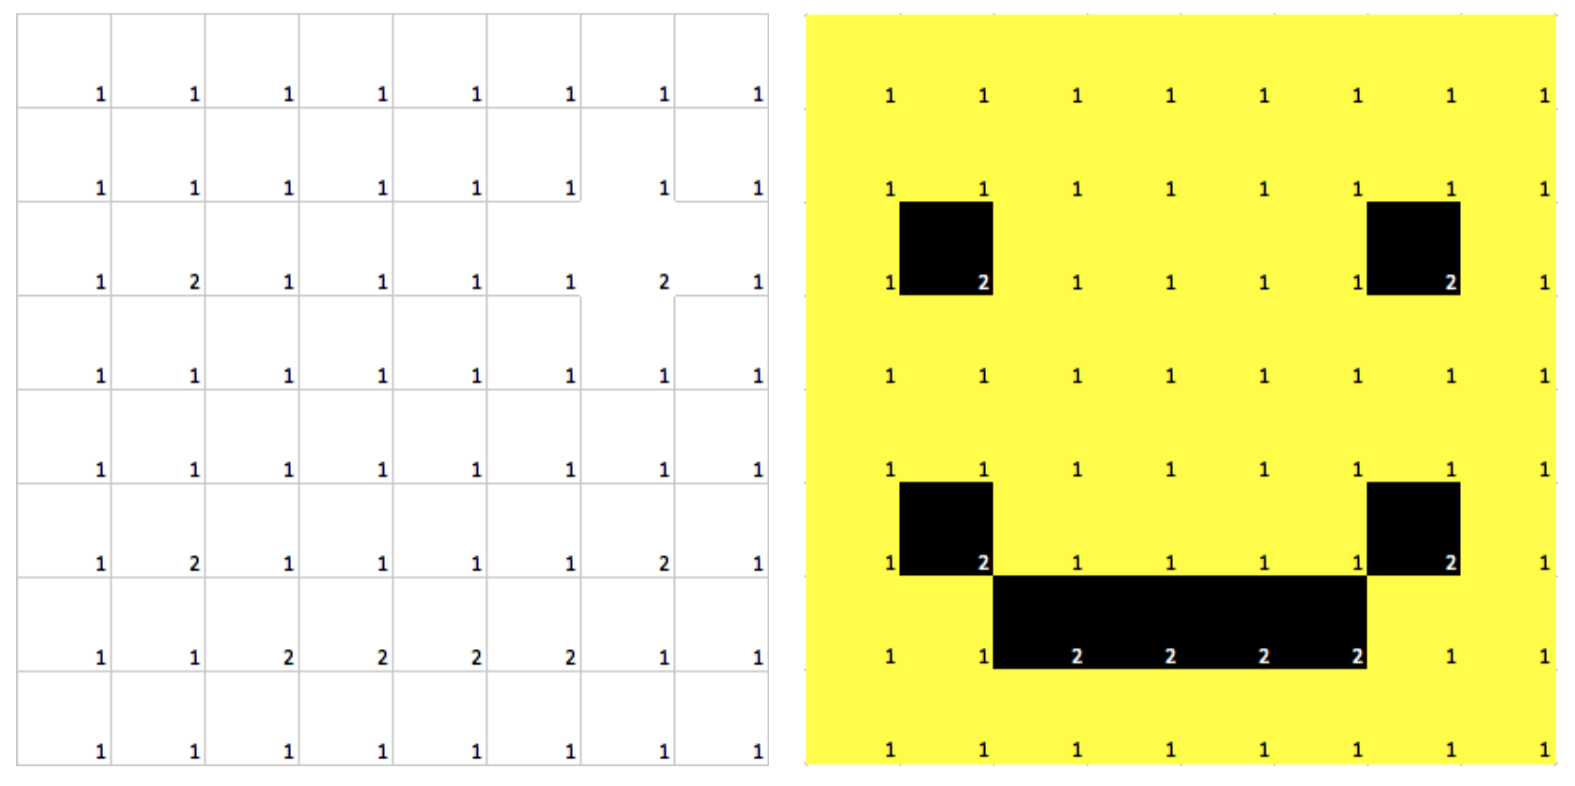
\includegraphics{images/screenshots/smiley.png}
\caption{A table of numbers on the left, and a color-coded table on the right, where the 2's have been highlighted in yellow. With the color, a pattern emerges that was not easy to see without the graphic. Figure used with permission from Correll (2015).}
\label{fig:smiley}
\end{figure}

While visualizations have many advantages, they can also be used to mislead, sometimes intentionally, and sometimes not (Correll, 2015; Kosslyn, 2006; Pandey, Rall, Satterthwaite, Nov, \& Bertini, 2015). For example, when means/standard errors are presented as barcharts, people tend to judge values below the mean (i.e., within the confines of the bar) as far more likely than values above the mean, even when the underlying distribution is symmetric (Correll, 2015). To further complicate matters, the default images in most point-and-click statistical software violate important visualization heuristics (Fife, Tremoulet, \& Longo, 2019; Healy \& Moody, 2014; Wainer, 2010). For example, in \texttt{SPSS} it is impossible (as far as I know) to produce standard error plots that display raw data (jittered or otherwise). Also, in standard error plots, the axes are scaled to the means, not the range of the actual data, which visually inflates the size of the effect. In addition, producing some types of graphics (e.g., Skew-Location plots) requires more effort than many are willing to perform (the user must model the data, export the residuals, then produce a scatterplot).

This paper introduces \texttt{flexplot}, an R package specifically designed to remove obstacles to sound visualizations. The graphics produced by \texttt{flexplot} were developed using empirically-derived heurstics (see Fife, Longo, Correll, \& Tremoulet, 2020 for a review). Also, the graphics produced are simple to generate and permit analysts to quickly shift between statistical modeling and graphical interpretation.

In the following section, I begin by outlining the guiding philosophy behind \texttt{flexplot}, then introduce its grammar. I then spend the remainder of the paper demonstrating how to produce intuitive graphics with \texttt{flexplot} and illustrate how to pair these tools with statistical modeling.

\hypertarget{guiding-philosophy-of-flexplot}{%
\section{Guiding Philosophy of Flexplot}\label{guiding-philosophy-of-flexplot}}

The traditional approach to data analysis requires a great deal of decision-making up-front, but requires little effort to interpret results. Initially, the analyst must choose between regression, ANOVA, \(t\)-tests, MANOVA, etc. If the analyst then chooses to graph these results, they must \emph{again} decide whether a boxplot, histogram, bar chart, scatterplot, etc. is most appropriate. By the time the analyst interprets the data, a great deal of effort has already been expended, though the traditional approach to data-analysis makes interpreting the results unambiguous; one simply needs to determine whether the p-value dips below the critical 0.05 threshold.

This approach has been routinely criticized (Cohen, 1994; Gigerenzer, 2004; Tyron, 1998), particularly in how results are interpreted (significant versus not). While the traditional approach requires great effort to choose the analysis and little effort to interpret it, \texttt{flexplot} takes the opposite approach: little effort is required to \emph{choose} the analysis, leaving more resources to \emph{interpret} the analysis. This is as it should be.

To accomplish this goal, \texttt{flexplot} is based on the following principles (Fife, Longo, Correll, \& Tremoulet, 2020):

\emph{1. Minimize obstacles to producing graphics.} The easier it is to produce graphics, the more likely they will be used, and the more resources the researcher will have available to interpret the results. Technology companies spend millions of dollars attempting to make the interaction between humans and technology as seamless as possible. One-click purchasing, voice-activated personal assistants like Siri, movies-on-demand, and audible app notifications are all innovations that are successful because they make it easy for humans to use their technology. Likewise, if producing a graphic is as simple (or simpler) than performing a statistical analysis, they too will become heavily utilized (and, dare I say, addictive?). Furthermore, the less effort required to produce them, the more resources available to invest in \emph{interpreting} graphics. To make producing graphics as simple as possible, \texttt{flexplot} automates much of the decision-making in the background, such as choosing between types of graphics (e.g., histograms versus bar charts) and how those graphics are displayed.

\emph{2. Design graphics that leverage human strenths and mitigate human biases.} Successful technology capitalizes on human strengths. A mobile phone, for example, leverages our advanced finger tactile sensitivity and dexterity. Sending text messages with one's toes would be a very poor choice. Likewise, a computer that sends olefactory information might work well for a dog, but not a human. Visualization technology ought to be designed with the same principles in mind. Unfortunately, standard statistical analyses do not capitalize on human strengths. It takes a great deal of training to understand even basic statistics, and even then results are frequently misinterpreted (Gigerenzer, 2004). To put it in the words of Tyron (1998), traditional analyses have a ``human factors'' problem. To overcome misconceptions about statistical analyses, some of the tools within \texttt{flexplot} create visual representations of the statistical models. These representations highlight uncertainty, reveal whether chosen models are appropriate, and improve encoding of statistical information.

\hypertarget{ggplot2-versus-flexplot}{%
\section{\texorpdfstring{\texttt{ggplot2} Versus \texttt{flexplot}}{ggplot2 Versus flexplot}}\label{ggplot2-versus-flexplot}}

Hadley Wickham, the author of \texttt{ggplot2}, developed a grammar of graphics (Wickham, 2010), or a set of rules that guide the construction of visualizations. Furthermore, Wickham's grammar is ``layered,'' which means that plotting elements can be stacked atop one another. For example, one could ``layer'' dots over an \(X/Y\) axis, layer a regression line over the dots, layer a correlation coefficient over the regression line, etc. Wickham's grammar allows a great deal of flexibility in the design of graphics. However, this flexibility comes at a cost. Very often the grammar necessary to produce a graphic requires a great deal of coding to produce. For example, consider the code to create jittered mean plots:

\small

\begin{Shaded}
\begin{Highlighting}[]
\FunctionTok{require}\NormalTok{(ggplot2)}
\FunctionTok{require}\NormalTok{(flexplot)}
\NormalTok{plot }\OtherTok{=} \FunctionTok{ggplot}\NormalTok{(}\AttributeTok{data =}\NormalTok{ exercise\_data, }\FunctionTok{aes}\NormalTok{(}\AttributeTok{x=}\NormalTok{therapy.type, }\AttributeTok{y=}\NormalTok{weight.loss)) }\SpecialCharTok{+} 
      \CommentTok{\# x/y axis layer}
  \FunctionTok{geom\_jitter}\NormalTok{(}\AttributeTok{width =}\NormalTok{ .}\DecValTok{2}\NormalTok{, }\AttributeTok{alpha =}\NormalTok{ .}\DecValTok{4}\NormalTok{) }\SpecialCharTok{+} 
      \CommentTok{\# point layer}
  \FunctionTok{stat\_summary}\NormalTok{(}\AttributeTok{fun.y =} \StringTok{\textquotesingle{}mean\textquotesingle{}}\NormalTok{, }\AttributeTok{geom =} \StringTok{\textquotesingle{}point\textquotesingle{}}\NormalTok{, }
        \AttributeTok{size =} \DecValTok{3}\NormalTok{, }\AttributeTok{position =} \FunctionTok{position\_dodge}\NormalTok{(}\AttributeTok{width =}\NormalTok{ .}\DecValTok{2}\NormalTok{)) }\SpecialCharTok{+} 
      \CommentTok{\# summary point layer}
  \FunctionTok{stat\_summary}\NormalTok{(}\AttributeTok{geom =} \StringTok{\textquotesingle{}errorbar\textquotesingle{}}\NormalTok{, }\AttributeTok{fun.ymin =} \ControlFlowTok{function}\NormalTok{(z)\{}\FunctionTok{mean}\NormalTok{(z)}\SpecialCharTok{{-}}\FloatTok{1.96}\SpecialCharTok{*}\FunctionTok{sd}\NormalTok{(z)\}, }
        \AttributeTok{fun.ymax=}\ControlFlowTok{function}\NormalTok{(z) \{}\FunctionTok{mean}\NormalTok{(z)}\SpecialCharTok{+}\FloatTok{1.96}\SpecialCharTok{*}\FunctionTok{sd}\NormalTok{(z)\}, }
        \AttributeTok{size =} \FloatTok{1.25}\NormalTok{, }\AttributeTok{width =}\NormalTok{ .}\DecValTok{2}\NormalTok{, }\AttributeTok{position =} \FunctionTok{position\_dodge}\NormalTok{(}\AttributeTok{width =}\NormalTok{ .}\DecValTok{2}\NormalTok{))  }
      \CommentTok{\# "errorbar" layer}
\end{Highlighting}
\end{Shaded}

\normalsize

I have personally spoken to many veteren R users who have been extremely reluctant to adopt \texttt{ggplot2}, simply because the approach and sytax are elaborate, if not complicated. For those less experienced, the prospect of leveraging \texttt{ggplot2} is even more daunting, which means that few will likely abandon point-and-click software to produce graphics.

As noted earlier, the more difficult it is to produce a graphic, the more likely it is someone will simply not use it. A similar graphic can be produced with only one line of code using the \texttt{flexplot} function:

\small

\begin{Shaded}
\begin{Highlighting}[]
\NormalTok{plot }\OtherTok{=} \FunctionTok{flexplot}\NormalTok{(weight.loss }\SpecialCharTok{\textasciitilde{}}\NormalTok{ therapy.type, }\AttributeTok{data =}\NormalTok{ exercise\_data)}
\end{Highlighting}
\end{Shaded}

\normalsize

Naturally, this simplicity comes at a cost; \texttt{flexplot} is more limited than \texttt{ggplot2}. However, it was not designed to be able to produce any graphic conceivable. Rather it was designed to visualize statistical models with ease, and will cover the majority of graphics analysts will use for modeling. However, in the end, graphics produced through \texttt{flexplot} are still \texttt{ggplot2} objects. As such, they can be edited and/or layered for further customization, which I will demonstrate throughout this paper.

\hypertarget{the-grammar-of-the-general-linear-model}{%
\section{The Grammar of the General Linear Model}\label{the-grammar-of-the-general-linear-model}}

\texttt{flexplot}'s grammar is also a layered grammar (but incidentally, because it was developed within \texttt{ggplot2}'s grammar), though its grammar is actually based on the linear model (LM).\footnote{The package \texttt{vizreg} (Breheny \& Burchett, 2017) is another R package that provides seamless integration with linear models.} Recall that most statistical procedures are subsumed within the LM, which is essentially regression. For example, a \(t\)-test is simply a regression where the intercept is the mean of the referent group (e.g., the control group) and the slope is simply the difference between the treatment and control groups. The base \texttt{R} function \texttt{lm} utilizes LMs to do various sorts of modeling, and all this is accomplished using a simple formula (e.g., \texttt{y\ \textasciitilde{}\ x1\ +\ x2}). Likewise, \texttt{flexplot} adopts the same convention, utilizing a similar formula to produce graphics. The advantage of this approach is that there is notational consistency from modeling to visualization. Very often the exact code used to produce a fitted model can also be used to visualize the data, as in the following example:

\small

\begin{Shaded}
\begin{Highlighting}[]
\NormalTok{model }\OtherTok{=}       \FunctionTok{lm}\NormalTok{(A }\SpecialCharTok{\textasciitilde{}}\NormalTok{ B }\SpecialCharTok{+}\NormalTok{ C, }\AttributeTok{data =}\NormalTok{ d)}
\NormalTok{plot  }\OtherTok{=} \FunctionTok{flexplot}\NormalTok{(A }\SpecialCharTok{\textasciitilde{}}\NormalTok{ B }\SpecialCharTok{+}\NormalTok{ C, }\AttributeTok{data =}\NormalTok{ d)}
\end{Highlighting}
\end{Shaded}

\normalsize

This simplifies the choice of graphics immensely; one only needs to specify the predictor variable(s) (and sometimes make some choices of paneling). Otherwise, \texttt{flexplot} handles the decision-making in the background.

Figure \ref{fig:flexplotgrammar} is an illustration that identifies which components of a \texttt{flexplot} equation produce each element of a \texttt{flexplot}-style graphic. The first variable in the equation (\(X1\)) specifies which variable is displayed on the \(X\) axis. The second variable (\(X2\)) is displayed as different colors/symbols/lines. The third and fourth elements are shown as column and row panels, respectively.

By following the grammar of a LM, there is consistency between statistical modeling and graphing, with a few notable exceptions. Most obviously, a LM formula (e.g., \texttt{plot(y\ \textasciitilde{}\ x1\ +\ x2\ +\ x3,\ data\ =\ data)}) does not have any vertical pipes (\texttt{\textbar{}}) as \texttt{flexplot} does (though other modeling procedures and R packages do, such as mixed models in \texttt{lmer}; coplots in the \texttt{car} packages; and the \texttt{visreg} package). The vertical pipe is necessary in \texttt{flexplot} to allow more specificity in paneling. Additionally, with LMs, one must explicitly specify interaction (e.g., \texttt{X1:X2}) and polynomial terms (e.g., \texttt{I(X2\^{}2)}). This is not necessary with \texttt{flexplot}; the raw data are displayed exactly as they are and if interactions are present, the graph will show it.

\begin{figure}
\centering
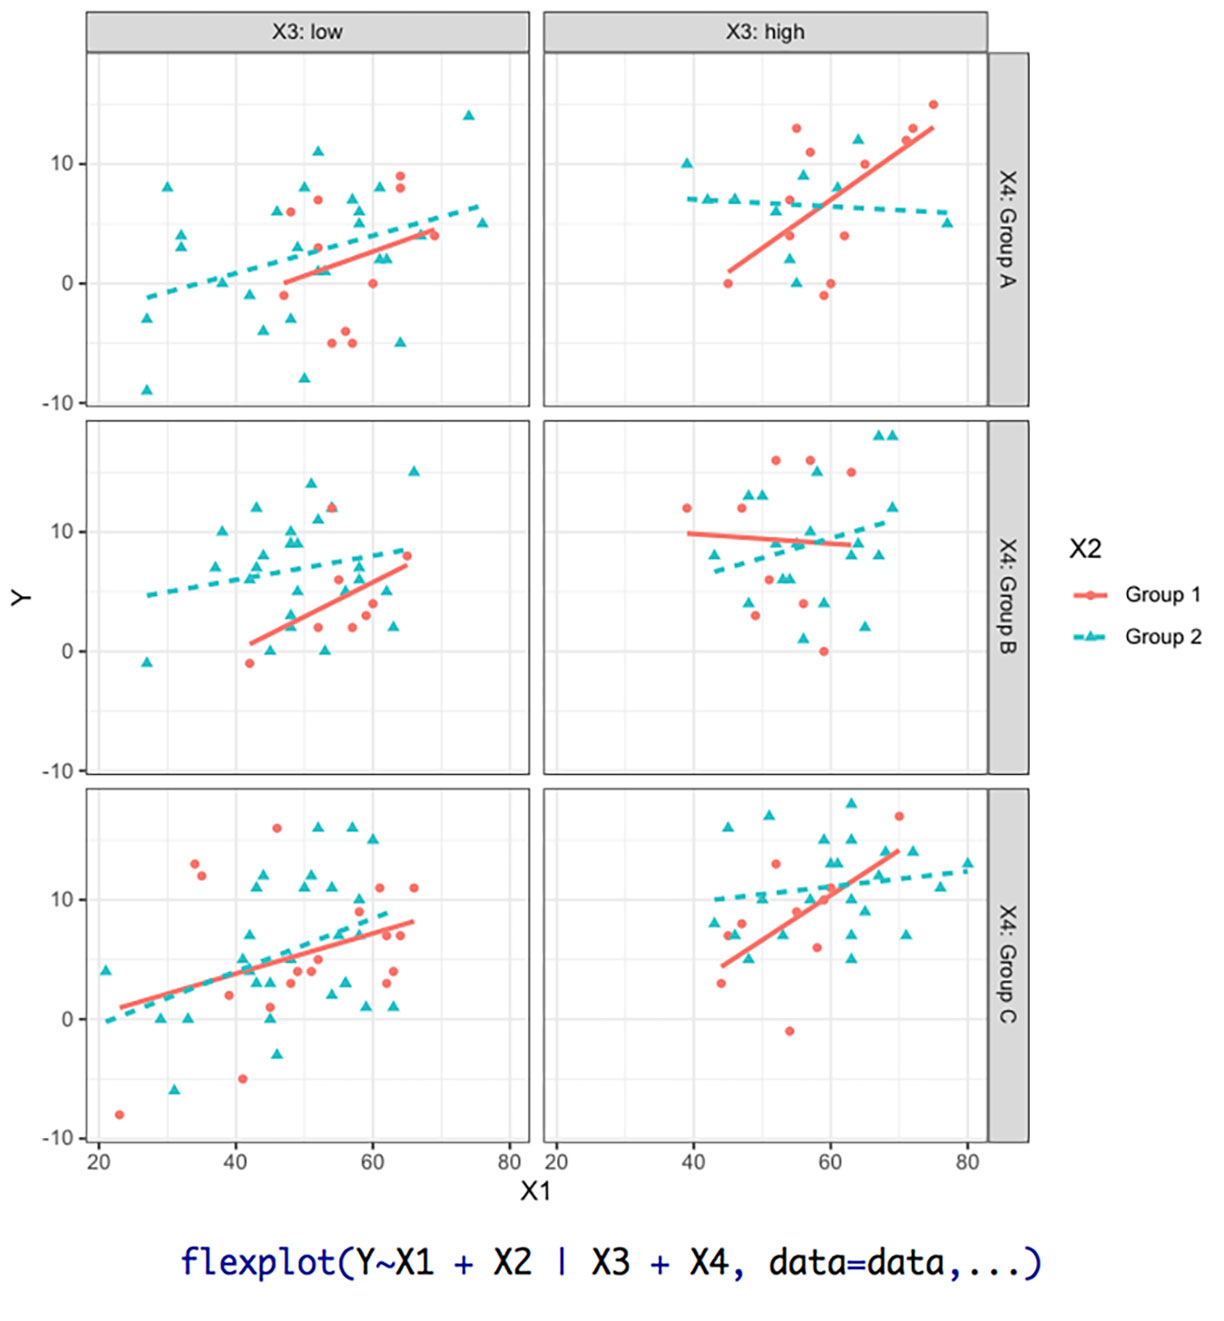
\includegraphics{images/flexplot_diagram.jpg}
\caption{A diagram showing how elements of Flexplot's graphics are represented in a plot. $X1$ is shown on the $X$ axis, $X2$ shows up as different colors/symbols/lines, $X3$ panels in columns, and $X4$ panels in rows.}
\label{fig:flexplotgrammar}
\end{figure}

The base \texttt{plot()} function in \texttt{R} follows similar conventions as \texttt{flexplot} (i.e., users can specify a formula, such as \texttt{plot(y\ \ \textasciitilde{}\ \ x)}), though \texttt{flexplot} is more intelligent in its choice of displays.\footnote{R's \texttt{plot()} function is a S3 method, so it is actually offers a great deal of flexibility for visualizing all sorts of R objects, much like flexplot's \texttt{visualize()} method. However, its flexibility is limited to package developers who must create a class to leverage the \texttt{plot()} method. The point I'm making here is not about the S3 \texttt{plot()} method, but about R's generic \texttt{plot()} function.} Also, \texttt{plot()} only allows the user to visualize one variable at a time. Another function, \texttt{coplot()}, allows some multivariate visualizations, yet it is limited in the types of data allowed and, like \texttt{plot()} is not flexible in the types of visualization decisions it makes. The \texttt{flexplot} package, on the other hand, offers great flexibility and automates much of the decision-making.

In the following section, I will demonstrate how decisions are made in \texttt{flexplot}. I begin by showing how to produce univariate graphics, then bivariate graphics, then multivariate graphics. I will then follow that up with various functions and techniques for combining graphs with models, then conclude with a brief summary.

\hypertarget{univariate-graphics}{%
\section{Univariate Graphics}\label{univariate-graphics}}

In \texttt{lm()}, one can fit an ``intercept only'' model, using the code \texttt{lm(y\ \textasciitilde{}\ 1)}. This is equivalent to estimating the mean of \(y\). \texttt{flexplot} follows a similar convention for graphing univariate distributions. Alternatively, one can also write this as \texttt{flexplot(y\textasciitilde{}y,\ ...)}. The type of graphic displayed depends on the type of variable inputted into the function. \texttt{flexplot} graphs numeric variables in histograms and categorical variables as barcharts. For example, in the code below, notice that \texttt{flexplot} recognizes whether the variable is categorical or numeric, and plots accordingly (see Figure \ref{fig:bar}).

\small

\begin{Shaded}
\begin{Highlighting}[]
\FunctionTok{require}\NormalTok{(patchwork) }\DocumentationTok{\#\#\#\# for combining plots into one}
\FunctionTok{require}\NormalTok{(flexplot)}
\FunctionTok{data}\NormalTok{(exercise\_data) }\DocumentationTok{\#\#\#\# these are simulated data available }
                    \DocumentationTok{\#\#\#\# in flexplot. }
\NormalTok{a }\OtherTok{=} \FunctionTok{flexplot}\NormalTok{(weight.loss }\SpecialCharTok{\textasciitilde{}} \DecValTok{1}\NormalTok{, }\AttributeTok{data =}\NormalTok{ exercise\_data)}
\NormalTok{b }\OtherTok{=} \FunctionTok{flexplot}\NormalTok{(therapy.type }\SpecialCharTok{\textasciitilde{}} \DecValTok{1}\NormalTok{, }\AttributeTok{data =}\NormalTok{ exercise\_data)}
\NormalTok{a }\SpecialCharTok{+}\NormalTok{ b}
\end{Highlighting}
\end{Shaded}

\begin{figure}
\centering
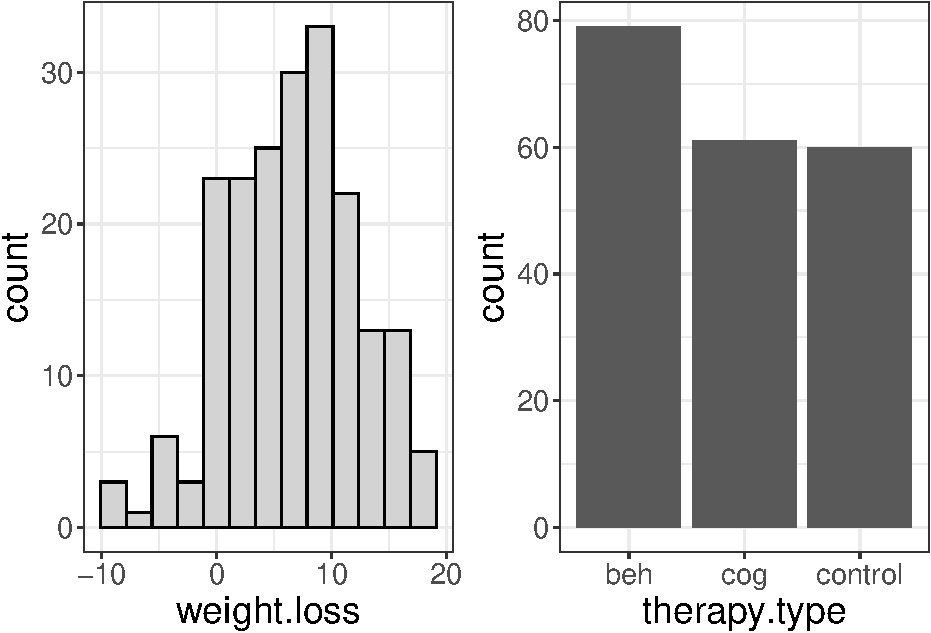
\includegraphics{flexplot_psychmeth_files/figure-latex/bar-1.pdf}
\caption{\label{fig:bar}A histogram (left) and barchart (right) produced within \texttt{flexplot} in R.}
\end{figure}

\normalsize

\texttt{flexplot} follows standard conventions when producing histograms. When producing barcharts, on the other hand, \texttt{flexplot} deviates from defaults. The order of the x-axis is typically sorted alphabetically in \texttt{ggplot2}, which violates the ``principle of relevance'' for visual processing (Kosslyn, 2006). This principle suggests that all features of a graphic should present meaningful information. Humans are primed to attend to visual differences, and stacking large and small \(N\) categories side-by-side willy nilly taxes the visual processing system into believing these differences are meaningful. \texttt{flexplot} automatically sorts the categories by sample size (the category with the largest \(N\) is left-most on the \(X\) axis), which also enhances the ability to ``chunk'' pieces of information meaningfully (Kosslyn, 2006), as in Figure \ref{fig:chunkit}. If the categories do have a meaningful order (e.g., if the variables are ordinal), the user can convert the variable of interest to an ordered factor.

\small

\begin{figure}
\centering
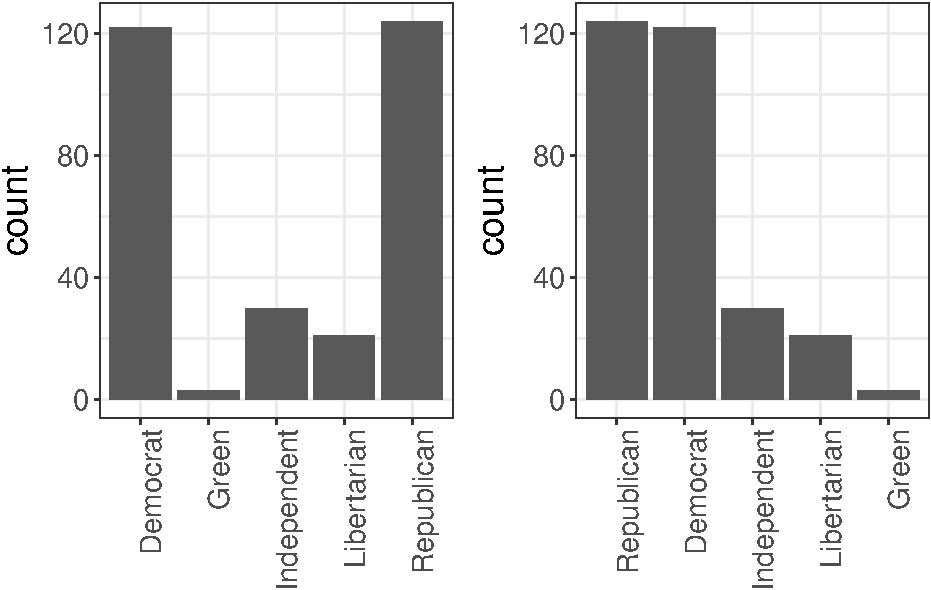
\includegraphics{flexplot_psychmeth_files/figure-latex/chunkit-1.pdf}
\caption{\label{fig:chunkit}Two displays of the same data. In the left image, categories are sorted alphabetically (which is the default of \texttt{ggplot2}). In \texttt{flexplot} the categories are sorted by sample size, which enables better chunking of information. \label{fig:chunkit}}
\end{figure}

\normalsize

Sometimes, \texttt{flexplot} will make a wrong guess, if, for example, a categorical variable is recorded as a number (e.g., 1 = Group 1, 2 = Group 2, 3 = Group 3). To force \texttt{flexplot} to produce a barchart, one can either convert the variable to a factor (e.g., \texttt{data\$group\ =\ factor(data\$group,\ levels\ =\ 1:3,\ labels\ =\ c("Group1",\ "Group2",\ "Group3"))}). Alternatively, one can use the \texttt{factor} function within a \texttt{flexplot} function (e.g., \texttt{flexplot(y\textasciitilde{}factor(group),\ data=d)}).

\hypertarget{bivariate-graphics}{%
\section{Bivariate Graphics}\label{bivariate-graphics}}

As with univariate graphics, \texttt{flexplot} will automatically produce an appropriate bivariate graphic, depending on the type of predictors and outcome variable: a numeric predictor/outcome will produce a scatterplot, a numeric predictor/categorical outcome = logistic curve graph, categorical predictor/numeric outcome = beeswarm plot, and categorical predictor/categorical outcome = association plot.

With all graphics produced by \texttt{flexplot} it will display the raw data. Although Tufte (2001) advocated for plots that minimize the ``data to ink ratio,'' subsequent investigation of visual perception have shown little evidence that minimizing ink in a graph improves visual perception (Inbar, Tractinsky, \& Meyer, 2007). Rather, raw data is essential for sound visual interpretation. Vastly different patterns can produce identical summary statistics such as means, variances, slopes, intercepts, etc. (Anscombe, 1973). Raw data allow one to determine, at a glance whether these summary statistics accurately reflect the raw data. Furthermore, research has shown that humans are quite adept at visually aggregating information from raw data without summary information (see Correll, 2015 for a review), while they cannot accurately surmise raw data from summary statistics. In other words, if anything is to be omitted, it should be the summary statistics (e.g., regression lines, whiskers in a boxplot, dots of means), not the raw data.

Visualizing raw data can become tricky, particularly when categorical variables are involved. With categorical variables, there is bound to be a great deal of overlap (e.g., if the treatment group has 100 participants, 100 individuals will have identical scores on the \(X\) axis when plotted, which will tend to mean datapoints will overlap). In the next section, I will explain how \texttt{flexplot} handles overlapping datapoints from categorical predictors.

\hypertarget{categorical-predictor-numeric-outcome-beeswarm-plots}{%
\subsection{Categorical Predictor, Numeric Outcome (Beeswarm Plots)}\label{categorical-predictor-numeric-outcome-beeswarm-plots}}

There are many different ways to graph a categorical predictor/numeric outcome relationship, including bar plots of means, box plots, violin plots, gradient plots, etc. Some are misleading (e.g., barplots of means and standard error plots). Others are mediocre (e.g., boxplots). Finally, some perform exceptionally well in human testing, including violin plots and gradient plots (Correll, 2015). As mentioned in the previous section, raw data are essential. To minimize overlap, a common strategy is to utilize ``jittering,'' which means that categorical variables are first converted to values (e.g., control group = 1, treatment group = 2), then random noise is added to each participant's score (e.g., a 1 may become 1.012 or 0.097). This reduces overlap between datapoints. However, simply jittering values uniformly robs one of a valuable opportunity to convey additional information in a graphic. \texttt{flexplot} instead jitters data proportional to the density of the data. In other words, regions of little density will have very little jittering and regions of high density (e.g., at the mode) will have more jittering. These sorts of plots are essentially violin plots with raw data, where the maximum amount of jittering is the outline of the violin plot. Traditionally, these were called ``textured dot strips,'' which were invented by Tukey and Tukey (1990; see also Wilkinson, 1999). Others (e.g., Eklund, 2012) call them ``bee swarm'' plots. I am not too fond of the original name, so I'll refer to them as bee swarm plots throughout this text.

While violin plots partially solve the problem mentioned earlier (i.e., that summary statistics can be generated from a diverse set of patterns of raw data), they too have their limitations. For one, it is impossible to tell the difference between a dataset with 15,000 versus 15 observations. For example, the two distributions in the left image in Figure \ref{fig:raw} look essentially the same, while the same data, plotted as beeswarm plots, very clearly show the sample size.

\small

\begin{Shaded}
\begin{Highlighting}[]
\NormalTok{group1 }\OtherTok{=} \FunctionTok{c}\NormalTok{(}\DecValTok{0}\NormalTok{,}\DecValTok{1}\NormalTok{,}\DecValTok{2}\NormalTok{,}\DecValTok{2}\NormalTok{,}\DecValTok{3}\NormalTok{,}\DecValTok{3}\NormalTok{,}\DecValTok{3}\NormalTok{,}\DecValTok{3}\NormalTok{,}\DecValTok{3}\NormalTok{,}\DecValTok{3}\NormalTok{,}\DecValTok{4}\NormalTok{,}\DecValTok{4}\NormalTok{,}\DecValTok{5}\NormalTok{,}\DecValTok{6}\NormalTok{)}
\NormalTok{group2 }\OtherTok{=} \FunctionTok{rnorm}\NormalTok{(}\DecValTok{10000}\NormalTok{,}\DecValTok{3}\NormalTok{,}\DecValTok{1}\NormalTok{)}
\NormalTok{d }\OtherTok{=} \FunctionTok{data.frame}\NormalTok{(}\AttributeTok{score =} \FunctionTok{c}\NormalTok{(group1, group2), }
               \AttributeTok{group =} \FunctionTok{factor}\NormalTok{(}\FunctionTok{c}\NormalTok{(}\FunctionTok{rep}\NormalTok{(}\StringTok{"group 1"}\NormalTok{, }\AttributeTok{times =} \FunctionTok{length}\NormalTok{(group1)), }
                       \FunctionTok{rep}\NormalTok{(}\StringTok{"group 2"}\NormalTok{, }\AttributeTok{times =} \FunctionTok{length}\NormalTok{(group2))), }\AttributeTok{ordered=}\NormalTok{T))}
\NormalTok{a }\OtherTok{=}\NormalTok{ ggplot2}\SpecialCharTok{::}\FunctionTok{ggplot}\NormalTok{(}\AttributeTok{data =}\NormalTok{ d, }\FunctionTok{aes}\NormalTok{(}\AttributeTok{x =}\NormalTok{ group, }\AttributeTok{y =}\NormalTok{ score)) }\SpecialCharTok{+}  
  \FunctionTok{geom\_violin}\NormalTok{() }\SpecialCharTok{+} \FunctionTok{theme\_bw}\NormalTok{()}
\NormalTok{b }\OtherTok{=} \FunctionTok{flexplot}\NormalTok{(score }\SpecialCharTok{\textasciitilde{}}\NormalTok{ group, }\AttributeTok{data =}\NormalTok{ d)}
\NormalTok{a }\SpecialCharTok{+}\NormalTok{ b}
\end{Highlighting}
\end{Shaded}

\begin{figure}

{\centering 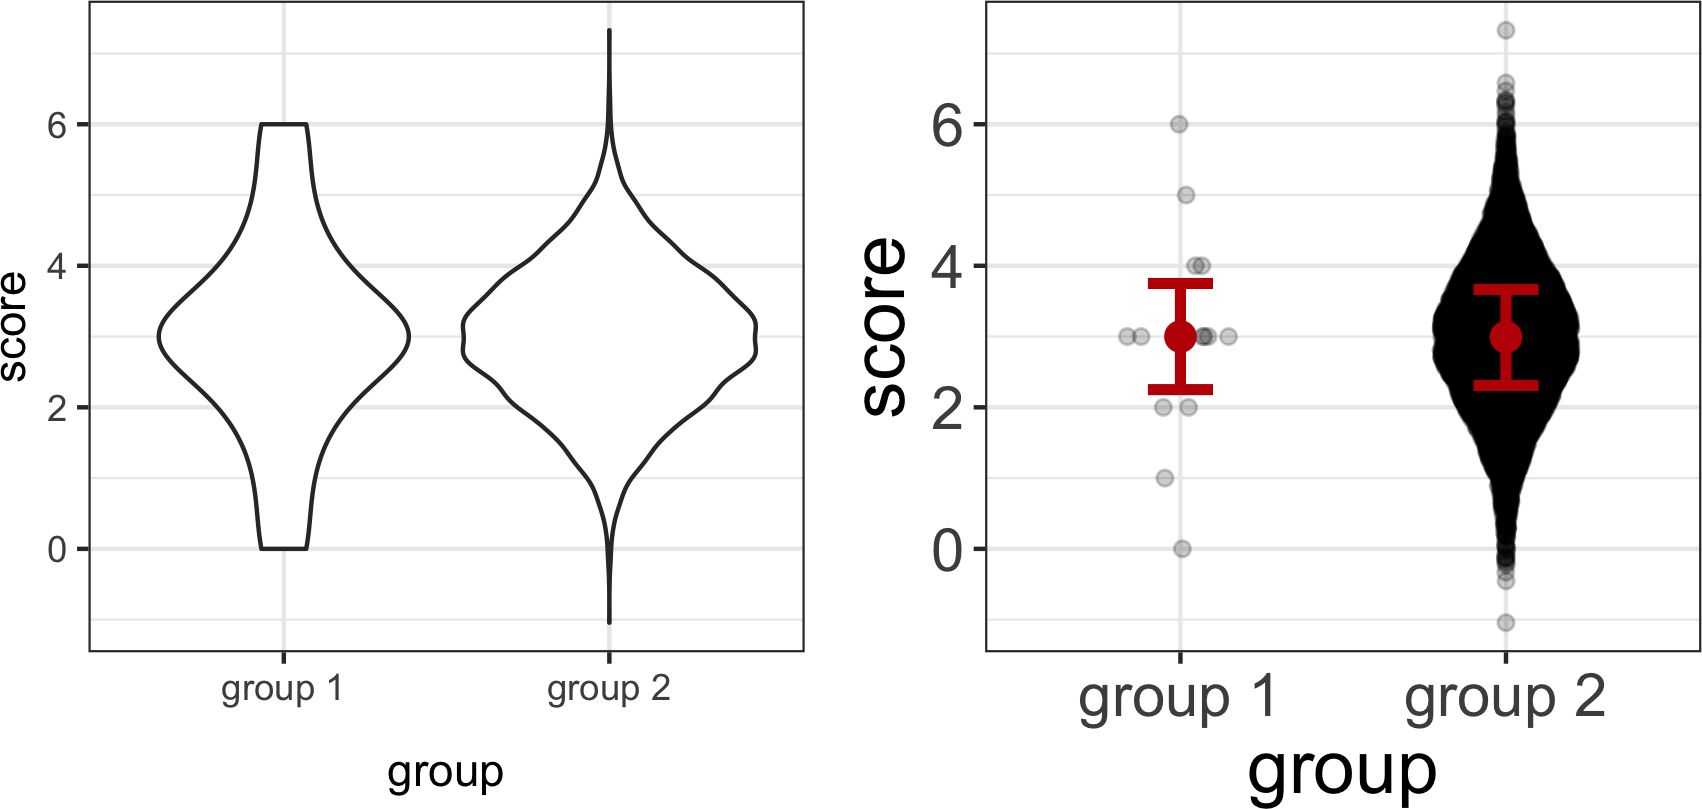
\includegraphics[width=0.9\linewidth]{flexplot_psychmeth_files/figure-latex/raw-1} 

}

\caption{Violin plots with 15,000 versus 15 datapoints. The outlines look the same in the left image, but the right image overlays the raw data, which makes the differing sample sizes much more apparent. \label{fig:raw}}\label{fig:raw}
\end{figure}

\normalsize

In \texttt{flexplot}, one can control the amount of jittering. The amount can be specified in multiple ways: as a boolean (\texttt{TRUE} means it will jitter, \texttt{FALSE} it will not), as a number (e.g., \texttt{0.2}), or as a vector (e.g., \texttt{c(.2,\ .4)}, which will indicate .2 jittering for X and .4 for Y). Just as it is in \texttt{geom\_jitter()}, this number refers to the amount of jittering on either side. However, the value refers to the \emph{maximum} amount the computer will jitter the data. So, 0.2 (the default) will jitter up to 0.1 points on the right, but only at the highest density and 0.1 on the left at the highest density.

Users can also specify what the ``whiskers'' mean for the summary statistics. They default to the interquartile range (with the median as the center dot), but the user can also specify \texttt{sterr}, or \texttt{stdev,} to indicate the standard error or standard deviation (see Figure \ref{fig:jitterit}):

\small

\begin{Shaded}
\begin{Highlighting}[]
\FunctionTok{theme\_update}\NormalTok{(}\AttributeTok{axis.text.x =} \FunctionTok{element\_text}\NormalTok{(}\AttributeTok{angle=}\DecValTok{90}\NormalTok{, }\AttributeTok{hjust=}\DecValTok{100}\NormalTok{))}
\NormalTok{a }\OtherTok{=} \FunctionTok{flexplot}\NormalTok{(weight.loss }\SpecialCharTok{\textasciitilde{}}\NormalTok{ therapy.type, }\AttributeTok{data =}\NormalTok{ exercise\_data, }
              \AttributeTok{jitter =}\NormalTok{ F, }\AttributeTok{spread =} \StringTok{"quartile"}\NormalTok{) }\SpecialCharTok{+}
              \FunctionTok{labs}\NormalTok{(}\AttributeTok{x=}\StringTok{""}\NormalTok{) }
\NormalTok{b }\OtherTok{=} \FunctionTok{flexplot}\NormalTok{(weight.loss }\SpecialCharTok{\textasciitilde{}}\NormalTok{ therapy.type, }\AttributeTok{data =}\NormalTok{ exercise\_data, }
              \AttributeTok{jitter =} \FunctionTok{c}\NormalTok{(.}\DecValTok{4}\NormalTok{,.}\DecValTok{5}\NormalTok{), }\AttributeTok{spread =} \StringTok{"sterr"}\NormalTok{) }\SpecialCharTok{+}
              \FunctionTok{labs}\NormalTok{(}\AttributeTok{x=}\StringTok{""}\NormalTok{)}
\NormalTok{c }\OtherTok{=} \FunctionTok{flexplot}\NormalTok{(weight.loss }\SpecialCharTok{\textasciitilde{}}\NormalTok{ therapy.type, }\AttributeTok{data =}\NormalTok{ exercise\_data, }
              \AttributeTok{jitter =}\NormalTok{ .}\DecValTok{2}\NormalTok{, }\AttributeTok{spread =} \StringTok{"stdev"}\NormalTok{) }\SpecialCharTok{+} 
              \FunctionTok{labs}\NormalTok{(}\AttributeTok{x=}\StringTok{""}\NormalTok{)}
\NormalTok{a }\SpecialCharTok{+}\NormalTok{ b }\SpecialCharTok{+}\NormalTok{ c }\SpecialCharTok{+} \FunctionTok{plot\_layout}\NormalTok{(}\AttributeTok{nrow =} \DecValTok{1}\NormalTok{)}
\end{Highlighting}
\end{Shaded}

\begin{figure}

{\centering 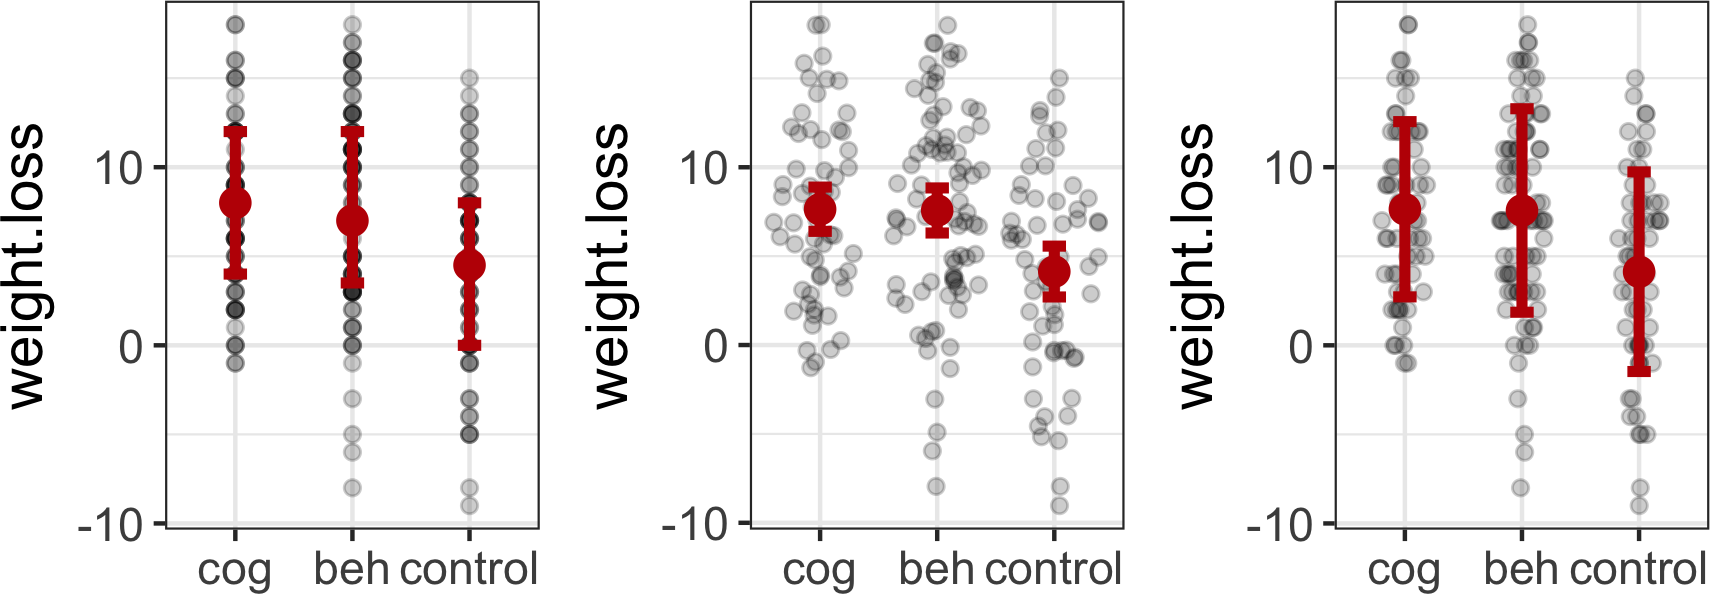
\includegraphics[width=0.9\linewidth]{flexplot_psychmeth_files/figure-latex/jitterit-1} 

}

\caption{Dot plots with the interquartile range and no jittering (left), beeswarm plot with mean + standard errors and jittering on $X$ and $Y$ (middle), and beeswarm plot with mean + standard deviation with jittering on only $X$ (right).}\label{fig:jitterit}
\end{figure}

\normalsize

\hypertarget{numeric-predictor-numeric-outcome-scatterplots}{%
\subsection{Numeric Predictor, Numeric Outcome (Scatterplots)}\label{numeric-predictor-numeric-outcome-scatterplots}}

The indisputed king of numeric on numeric visualization is the scatterplot. Once again, \texttt{flexplot} is smart enough to choose a scatterplot when it is passed a numeric predictor and numeric outcome. Except for severe departures, people tend to believe the fit of a line overlaid on raw data, even when the line is not appropriate (Fife, Tremoulet, \& Longo, 2019). For this reason, \texttt{flexplot} defaults to graphing a loess line as the summary statistic, so as to highlight deviations from linearity. However, the user can specify other sorts of fits, such as \texttt{"lm"} (for regression), \texttt{"quadratic"}, \texttt{"cubic"}, \texttt{"logistic"}, ``\texttt{poisson},'' ``\texttt{gamma},'' and \texttt{"rlm"} (robust linear model) in the \texttt{MASS} package (Ripley et al., 2013). The user can also choose to remove the confidence interval by specifying \texttt{se\ =\ F}, as well as jitter one or both variables, as shown below and in Figure \ref{fig:scatter}.

\small

\begin{Shaded}
\begin{Highlighting}[]
\NormalTok{a }\OtherTok{=} \FunctionTok{flexplot}\NormalTok{(weight.loss }\SpecialCharTok{\textasciitilde{}}\NormalTok{ satisfaction, }\AttributeTok{data =}\NormalTok{ exercise\_data) }\SpecialCharTok{+} 
  \FunctionTok{theme\_minimal}\NormalTok{() }\DocumentationTok{\#\#\# using layering to change theme}
\NormalTok{b }\OtherTok{=} \FunctionTok{flexplot}\NormalTok{(weight.loss }\SpecialCharTok{\textasciitilde{}}\NormalTok{ satisfaction, }\AttributeTok{data =}\NormalTok{ exercise\_data, }
             \AttributeTok{method =} \StringTok{"lm"}\NormalTok{, }\AttributeTok{se =}\NormalTok{ F)}
\NormalTok{c }\OtherTok{=} \FunctionTok{flexplot}\NormalTok{(weight.loss }\SpecialCharTok{\textasciitilde{}}\NormalTok{ satisfaction, }\AttributeTok{data =}\NormalTok{ exercise\_data, }
             \AttributeTok{method =} \StringTok{"polynomial"}\NormalTok{, }\AttributeTok{jitter =}\NormalTok{ .}\DecValTok{4}\NormalTok{)}
\NormalTok{a }\SpecialCharTok{+}\NormalTok{ b }\SpecialCharTok{+}\NormalTok{ c }\SpecialCharTok{+} \FunctionTok{plot\_layout}\NormalTok{(}\AttributeTok{nrow =} \DecValTok{1}\NormalTok{)}
\end{Highlighting}
\end{Shaded}

\begin{figure}

{\centering 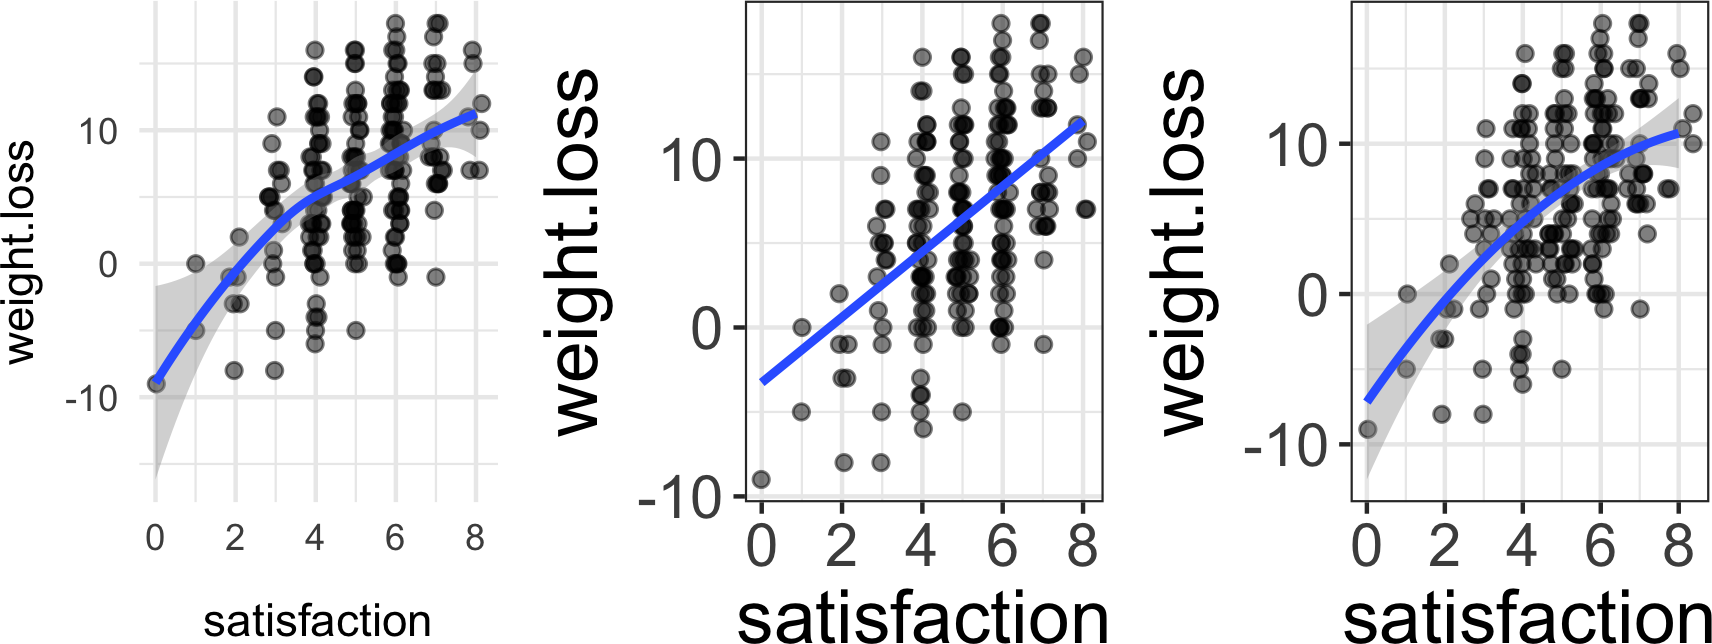
\includegraphics{flexplot_psychmeth_files/figure-latex/scatter-1} 

}

\caption{Scatterplot with different options of fit: loess (default), lm (regression), and quadratic Also, the data in the far right plot has been jittered. }\label{fig:scatter}
\end{figure}

\normalsize

Though \texttt{flexplot} defaults to a loess line, if the analyst models the data using another fitted function (e.g., regression, cubic, robust), the final display should reflect that (Umanath \& Vessey, 1994; Vessey, 1991). This process is seamless when one uses the \texttt{visualize} function, discussed shortly.

\hypertarget{numeric-predictor-categorical-outcome-logistic-curves}{%
\subsection{Numeric Predictor, Categorical Outcome (Logistic Curves)}\label{numeric-predictor-categorical-outcome-logistic-curves}}

\texttt{flexplot} also has some ability to model categorical outcomes. One common situation might be when one is attempting to model a binary outcome, as they would in a logistic regression. In this situation, it is critical that the graph match the analysis (Fife, 2020). This aligns with the principle of ``cognitive fit,'' which suggests that the type of display matches the type of information conveyed (Umanath \& Vessey, 1994; Vessey, 1991). Because logistic regressions utilize ogive curves to model the data, the graphs ought to reflect that.

Any binary variable can be graphed as a logistic regression in \texttt{flexplot}, except when the axis variable (i.e., the variable occupying the first slot in the \texttt{flexplot} equation) is also categorical. To model logistic curves, the user only needs to specify \texttt{logistic} as the method (see Figure \ref{fig:logistic}).

\small

\begin{Shaded}
\begin{Highlighting}[]
\FunctionTok{data}\NormalTok{(}\StringTok{"tablesaw.injury"}\NormalTok{) }\DocumentationTok{\#\#\# also simulated data available }
                        \DocumentationTok{\#\#\# in flexplot package}
\FunctionTok{flexplot}\NormalTok{(injury }\SpecialCharTok{\textasciitilde{}}\NormalTok{ attention, }\AttributeTok{data =}\NormalTok{ tablesaw.injury, }
             \AttributeTok{method =} \StringTok{"logistic"}\NormalTok{, }\AttributeTok{jitter =} \FunctionTok{c}\NormalTok{(}\DecValTok{0}\NormalTok{, .}\DecValTok{05}\NormalTok{))}
\end{Highlighting}
\end{Shaded}

\begin{figure}
\centering
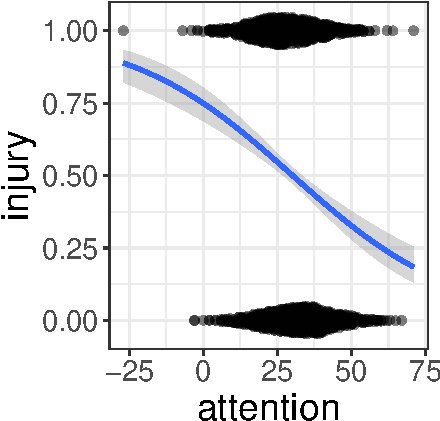
\includegraphics{flexplot_psychmeth_files/figure-latex/logistic-1.pdf}
\caption{\label{fig:logistic}Example of a logistic plot in the \texttt{flexplot} package.\label{fig:logistic}}
\end{figure}

\normalsize

\hypertarget{categorical-outcome-categorical-predictor-association-plots}{%
\subsection{Categorical Outcome, Categorical Predictor (Association Plots)}\label{categorical-outcome-categorical-predictor-association-plots}}

Sometimes the analyst may wish to graph the relationship between two categorical variables. Once again, \texttt{flexplot} is smart enough to determine that information from the formula, provided the user supplies two factors. In this situation, \texttt{flexplot} will generate an ``association'' plot, which plots the deviation of each cell from its expected frequencies (divided by the expected values within that cell). The reason for an association plot (as opposed to a traditional barplot) is because it best maps into what sorts of questions viewers are interested in asking. When users model the association between categorical variables, they traditionally use a \(\chi^2\) test, which compares observed versus expected frequencies. An association plot displays observed (height of bar) versus expected (y axis at zero) frequencies, thus following the principle of cognitive fit (Umanath \& Vessey, 1994; Vessey, 1991; see also Kosslyn, 2006 for a similar principle, the {``principle of compatibility''}).

In the example below, I had to convert \texttt{injury} to a factor to get a barplot. The graphic (Figure \ref{fig:association}) shows that females are less likely to be injured than males, relatively speaking.

\small

\begin{Shaded}
\begin{Highlighting}[]
\NormalTok{tablesaw.injury }\OtherTok{=} \FunctionTok{within}\NormalTok{(tablesaw.injury, \{injury }\OtherTok{=} \FunctionTok{factor}\NormalTok{(injury, }
                    \AttributeTok{levels=}\FunctionTok{c}\NormalTok{(}\DecValTok{0}\NormalTok{, }\DecValTok{1}\NormalTok{), }\AttributeTok{labels=}\FunctionTok{c}\NormalTok{(}\StringTok{"all good"}\NormalTok{, }\StringTok{"ouch"}\NormalTok{))\})}
\FunctionTok{flexplot}\NormalTok{(injury }\SpecialCharTok{\textasciitilde{}}\NormalTok{ gender, }\AttributeTok{data =}\NormalTok{ tablesaw.injury)}
\end{Highlighting}
\end{Shaded}

\begin{figure}
\centering
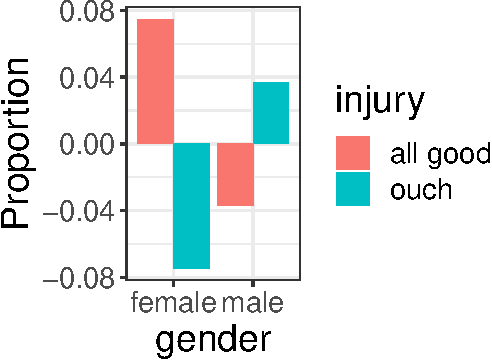
\includegraphics{flexplot_psychmeth_files/figure-latex/association-1.pdf}
\caption{\label{fig:association}Example of an association plot for categorical predictor/categorical outcome.\label{fig:association}}
\end{figure}

\normalsize

\hypertarget{repeated-measures-data-related-t-test}{%
\subsection{\texorpdfstring{Repeated Measures Data (Related \(t\)-test)}{Repeated Measures Data (Related t-test)}}\label{repeated-measures-data-related-t-test}}

One of the guiding tenets of \texttt{flexplot} is that every statistical analysis ought to be accompanied by a graphic that closely matches the analysis. This not only improves encoding of statistical information, but it also highlights uncertainty and reveals the appropriateness of the model. With a related \(t\)-test, the existing graphics will not accurately represent this model because a related \(t\) actually models the \emph{difference} between scores (e.g., from Time 1 to Time 2). As such, \texttt{flexplot} allows an additional option (\texttt{related\ =\ TRUE}) that tells \texttt{flexplot} to plot the differences, rather than the groups. To do so, \texttt{flexplot} requires ``tidy'' data, or data where time is indicated in one column and the score in the other. Also, there must be equal numbers of observations in each group. Once in this format, it simply plots the differences (Figure \ref{fig:plant}). For example:

\small

\begin{Shaded}
\begin{Highlighting}[]
\FunctionTok{data}\NormalTok{(}\StringTok{"plant\_growth"}\NormalTok{)}
\FunctionTok{flexplot}\NormalTok{(Diameter }\SpecialCharTok{\textasciitilde{}}\NormalTok{ Soil.Type, }\AttributeTok{data =}\NormalTok{ plant\_growth, }\AttributeTok{related=}\NormalTok{T) }\SpecialCharTok{+}
  \FunctionTok{theme}\NormalTok{(}\AttributeTok{axis.title=}\FunctionTok{element\_text}\NormalTok{(}\AttributeTok{size=}\DecValTok{12}\NormalTok{,}\AttributeTok{face=}\StringTok{"bold"}\NormalTok{))}
\end{Highlighting}
\end{Shaded}

\begin{figure}
\centering
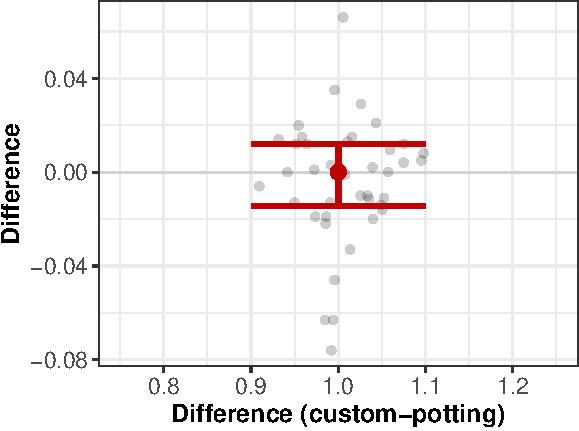
\includegraphics{flexplot_psychmeth_files/figure-latex/plant-1.pdf}
\caption{\label{fig:plant}A plot of repeated measures data.\label{fig:plant}}
\end{figure}

\normalsize

\noindent (Note, this dataset didn't actually contain repeated measures data. This is merely for illustrative purposes).

Unfortunately, plotting difference scores only works with two timepoints. When there are more than two timepoints, I recommend graphing these relationships with the \texttt{visualize()} function using mixed models. (I'll address \texttt{visualize()} shortly). In the plant growth graphic, the differences seem centered around zero, indicating that the type of potting soil used (store-bought potting soil versus a ``secret'' custom mix I found online) didn't make a difference in seedling diameter.

\hypertarget{avoiding-overlap}{%
\subsection{Avoiding Overlap}\label{avoiding-overlap}}

If it wasn't yet apparent, let me be less subtle: I think all graphics should include raw data. Showing raw data allows readers to determine whether the chosen model is appropriate, and it communicates the degree of uncertainty about the model. However, when there are a large number of datapoints, it increases cognitive load and masks salient characteristics (Kosslyn, 2006). This makes it quite difficult to see any patterns; areas of high density look just as crowded as areas of lower density, relatively speaking (although having bee swarm plots makes it clear which areas are most dense; see the example in top-left image in Figure \ref{fig:sample}). To address such overlap, \texttt{flexplot} offers three options (aside from making the plot bigger, of course). The first is to suppress raw data (\texttt{raw.data\ =\ F}, right-top in Figure \ref{fig:sample}). I don't recommend that, but it can be done.

A second option is to reduce the transparency (e.g., bottom-left in Figure \ref{fig:sample}). This will draw more attention to the fit of the model than the raw data (e.g., users will attend to the regression line rather than the raw data; see Kosslyn, 2006), which may or may not be a good thing. Perhaps the best option is to \emph{sample} (bottom-right in Figure \ref{fig:sample}). Sampling allows the visual-processing system to not be overly influenced by the fit, but without overwhelming the visual processing system. However, it is important that the visual display of fit (e.g., median + IQR, loess line, regression line) not be estimated from the sampled data. Rather, the fit should correspond to the entire dataset. \texttt{flexplot} performs this operation in the background. In Figure \ref{fig:sample}, notice how the medians/interquartile ranges do not change, despite having different numbers of datapoints.

\small

\begin{Shaded}
\begin{Highlighting}[]
\FunctionTok{data}\NormalTok{(}\StringTok{"nsduh"}\NormalTok{)}
\NormalTok{a }\OtherTok{=} \FunctionTok{flexplot}\NormalTok{(distress }\SpecialCharTok{\textasciitilde{}}\NormalTok{ major.dep, }\AttributeTok{data =}\NormalTok{ nsduh)}
\NormalTok{b }\OtherTok{=} \FunctionTok{flexplot}\NormalTok{(distress }\SpecialCharTok{\textasciitilde{}}\NormalTok{ major.dep, }\AttributeTok{data =}\NormalTok{ nsduh, }\AttributeTok{raw.data =}\NormalTok{ F)}
\NormalTok{c }\OtherTok{=} \FunctionTok{flexplot}\NormalTok{(distress }\SpecialCharTok{\textasciitilde{}}\NormalTok{ major.dep, }\AttributeTok{data =}\NormalTok{ nsduh, }\AttributeTok{alpha =}\NormalTok{ .}\DecValTok{005}\NormalTok{)}
\NormalTok{d }\OtherTok{=} \FunctionTok{flexplot}\NormalTok{(distress }\SpecialCharTok{\textasciitilde{}}\NormalTok{ major.dep, }\AttributeTok{data =}\NormalTok{ nsduh, }\AttributeTok{sample =} \DecValTok{200}\NormalTok{)}
\NormalTok{a }\SpecialCharTok{+}\NormalTok{ b }\SpecialCharTok{+}\NormalTok{ c }\SpecialCharTok{+}\NormalTok{ d }\SpecialCharTok{+} \FunctionTok{plot\_layout}\NormalTok{(}\AttributeTok{nrow =} \DecValTok{2}\NormalTok{)}
\end{Highlighting}
\end{Shaded}

\begin{figure}
\centering
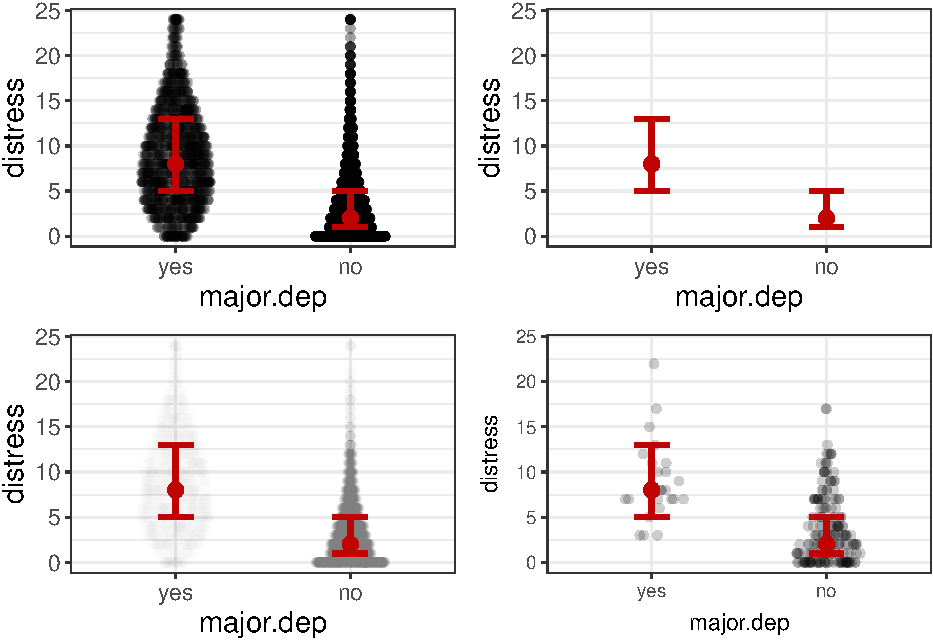
\includegraphics{flexplot_psychmeth_files/figure-latex/sample-1.pdf}
\caption{\label{fig:sample}Four graphics showing different ways to handle overlapping datapoints. The top-left image does nothing. The top-right omits raw data. The bottom-left reduces the opacity of the points. The bottom-right samples datapoints. \label{fig:sample}}
\end{figure}

\normalsize

\hypertarget{multivariate-graphics}{%
\section{Multivariate Graphics}\label{multivariate-graphics}}

Graphing multivariate relationships can become quite tricky. It is very easy to induce cognitive overload, especially when attempting to visualize raw data (which is, again, a key characteristic of \texttt{flexplot}). Some might be inclined to create three-dimensional plots. However, these are difficult to interpret and they require the user to rotate the view. Even then, they can only show two predictors at a time. I find it much easier to use other strategies. \texttt{flexplot} utilizes four different strategies to visualize multivariate relationships: (1) plotting a dimension as different colors/lines/shapes, (2) plotting a dimension in row or column panels, (3) visualizing conditional relationships with added variable plots, and (4) overlaying ghost lines.

\hypertarget{added-variable-plots-avps-with-added.plot}{%
\subsection{\texorpdfstring{Added Variable Plots (AVPs) With \texttt{added.plot()}}{Added Variable Plots (AVPs) With added.plot()}}\label{added-variable-plots-avps-with-added.plot}}

AVPs are underused, yet extremely useful.\footnote{The \texttt{car} package allows users to construct AVPs, but does so with R's native plots. This means one cannot leverage the advantages of \texttt{ggplot} (e.g., layering).} Essentially, an AVP shows the relationship between a predictor of interest and the \emph{residuals} of an existing model. (Alternatively, one can use partial residual plots, which are based on a similar principle. See Fife, 2021). For example, if one wanted to understand the relationship between \texttt{therapy.type} and \texttt{weight.loss} after controlling for \texttt{motivation}, that person could build a model predicting \texttt{weight.loss} from \texttt{motivation}, residualize that relationship, then show a beeswarm plot of the residuals for each type of therapy. This is what AVPs do (see Figure \ref{fig:avp}). These reduce cognitive load substantially, since users only need to interpret two dimensions.

\texttt{flexplot\textquotesingle{}s} version of AVPs have a slightly different flavor. In my experience, AVPs can be confusing to lay audiences because the scale of the outcome variable has changed to be centered on zero; if one is expecting the outcome variable to range from 0 to 30, yet the graph shows scores from -15 to +15, this will violate users' intuitions, which will create obstacles to proper interpretation of graphics (Kosslyn, 2006). To counter this confusion, \texttt{flexplot} adds the mean back into the residuals so the \(Y\)-axis retains the original scale. The notation for \texttt{added.plot()} is similar to \texttt{flexplot}, though the vertical pipes aren't necessary.

There are multiple ways to specify the display of added variable plots. By default, \texttt{flexplot} will do is take the \emph{last} variable entered (\texttt{therapy.type} in the first line of the code below) and plot that on the \(X\) axis, while plotting the residuals of the model on the \(Y\) axis (i.e., the residuals of the model \texttt{weight.loss\ \textasciitilde{}\ motivation}). Another option is to specify either a number (indicating the ordinal position of the variable they wish to plot on the \(X\) axis, as in the second example below) or the variable name in quotes (see the third line in the example code below). Other arguments can be passed to \texttt{added.plot()} as well (such as \texttt{alpha}, \texttt{sample}, \texttt{method}, etc.). A final option is to specify explicitly how the residuals are computed (using the \texttt{lm\_formula} argument), separately from how the data are displayed (via the formula argument). This final method allows one to specify a multivariate plot, as in Figure \ref{fig:avp}.

\begin{Shaded}
\begin{Highlighting}[]
\FunctionTok{added.plot}\NormalTok{(weight.loss }\SpecialCharTok{\textasciitilde{}}\NormalTok{ motivation }\SpecialCharTok{+}\NormalTok{ therapy.type, }\AttributeTok{data =}\NormalTok{ exercise\_data)}
\FunctionTok{added.plot}\NormalTok{(weight.loss }\SpecialCharTok{\textasciitilde{}}\NormalTok{ motivation }\SpecialCharTok{+}\NormalTok{ therapy.type, }\AttributeTok{data =}\NormalTok{ exercise\_data, }\AttributeTok{x=}\DecValTok{1}\NormalTok{) }
\FunctionTok{added.plot}\NormalTok{(weight.loss }\SpecialCharTok{\textasciitilde{}}\NormalTok{ motivation }\SpecialCharTok{+}\NormalTok{ therapy.type, }\AttributeTok{data =}\NormalTok{ exercise\_data, }\AttributeTok{x=}\StringTok{"motivation"}\NormalTok{) }
\FunctionTok{added.plot}\NormalTok{(weight.loss}\SpecialCharTok{\textasciitilde{}}\NormalTok{motivation }\SpecialCharTok{|}\NormalTok{ therapy.type, }\AttributeTok{data=}\NormalTok{exercise\_data, }
           \AttributeTok{lm\_formula =}\NormalTok{ weight.loss}\SpecialCharTok{\textasciitilde{}}\NormalTok{health)}
\end{Highlighting}
\end{Shaded}

\small

\begin{Shaded}
\begin{Highlighting}[]
\FunctionTok{added.plot}\NormalTok{(weight.loss}\SpecialCharTok{\textasciitilde{}}\NormalTok{motivation }\SpecialCharTok{|}\NormalTok{ therapy.type, }\AttributeTok{data=}\NormalTok{exercise\_data, }
           \AttributeTok{lm\_formula =}\NormalTok{ weight.loss}\SpecialCharTok{\textasciitilde{}}\NormalTok{health)}
\end{Highlighting}
\end{Shaded}

\normalsize

\hypertarget{colorslinesshapes}{%
\subsection{Colors/Lines/Shapes}\label{colorslinesshapes}}

As shown in Figure \ref{fig:flexplotgrammar}, the second slot in the \texttt{flexplot} formula (\texttt{X2} in Figure \ref{fig:flexplotgrammar}) controls which variable is displayed as different colors/symbols/lines. Figure \ref{fig:symbols} shows two examples of this: one where a numeric predictor is on the \(X\) axis, and one where a categorical predictor is on the X-axis. When categorical variables are shown on the \(X\) axis, \texttt{flexplot} draws lines connecting the medians (or means).

\small

\begin{Shaded}
\begin{Highlighting}[]
\NormalTok{a }\OtherTok{=} \FunctionTok{flexplot}\NormalTok{(weight.loss }\SpecialCharTok{\textasciitilde{}}\NormalTok{ motivation }\SpecialCharTok{+}\NormalTok{ gender, }
    \AttributeTok{data =}\NormalTok{ exercise\_data, }\AttributeTok{se =}\NormalTok{ F, }\AttributeTok{alpha =}\NormalTok{ .}\DecValTok{3}\NormalTok{)}
\NormalTok{b }\OtherTok{=} \FunctionTok{flexplot}\NormalTok{(weight.loss }\SpecialCharTok{\textasciitilde{}}\NormalTok{ therapy.type }\SpecialCharTok{+}\NormalTok{ gender, }
    \AttributeTok{data =}\NormalTok{ exercise\_data, }\AttributeTok{se =}\NormalTok{ F, }\AttributeTok{alpha =}\NormalTok{ .}\DecValTok{3}\NormalTok{) }\SpecialCharTok{+}
    \FunctionTok{theme}\NormalTok{(}\AttributeTok{axis.text.x =} \FunctionTok{element\_text}\NormalTok{(}\AttributeTok{angle=}\DecValTok{90}\NormalTok{, }\AttributeTok{hjust=}\DecValTok{1}\NormalTok{, }\AttributeTok{vjust=}\NormalTok{.}\DecValTok{2}\NormalTok{))}
\NormalTok{a }\SpecialCharTok{+}\NormalTok{ b}
\end{Highlighting}
\end{Shaded}

\begin{figure}
\centering
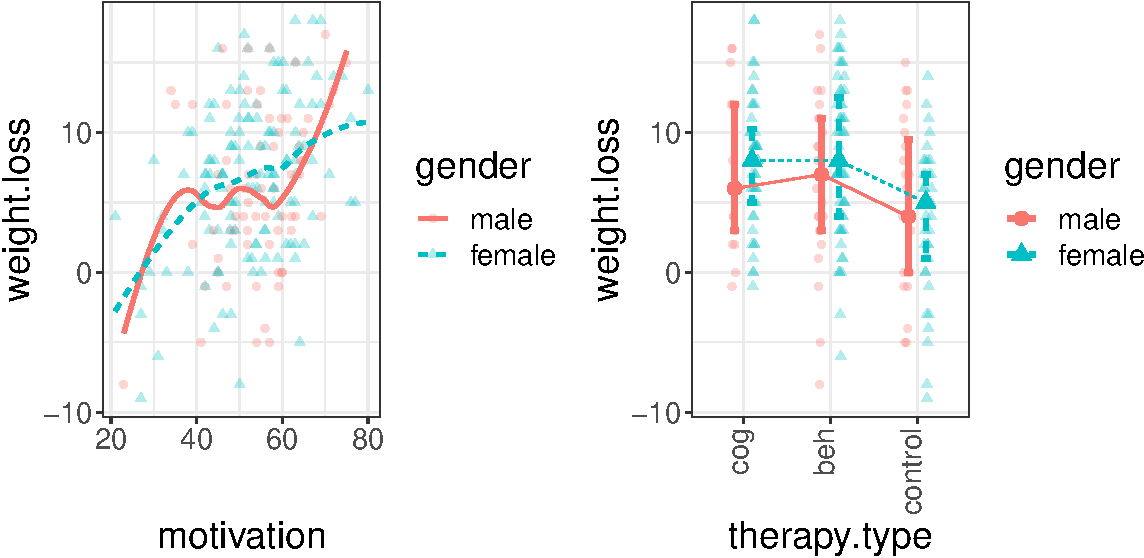
\includegraphics{flexplot_psychmeth_files/figure-latex/symbols-1.pdf}
\caption{\label{fig:symbols}Two multivariate graphs illustrating how the second slot in a \texttt{flexplot} formula controls the graph. The left image demonstrates what happens to the second slot variable (\(X2\)) when a numeric predictor is on the X-axis, while the right image demonstrates what happens to the second slot variable when a categorical predictor is on the X-axis.}
\end{figure}

\normalsize

One limitation of colors/shapes/symbols is the increase in cognitive load. When plotting different symbols/colors/lines on the same graph, there is often a great deal of overlap, which makes it more difficult to pick out patterns. While research suggests we can conceptualize up to four unique elements (Kosslyn, 2006), in my experience, having a variable with more than two levels in the second slot of a \texttt{flexplot} equation becomes challenging to interpret, particularly when there are more than a handful of datapoints.

\hypertarget{paneling}{%
\subsection{Paneling}\label{paneling}}

An alternative (or additional) strategy for plotting multivariate data is paneling. As shown in Figure \ref{fig:flexplotgrammar}, the third and fourth slots control paneling in columns and rows, respectively. The panels follow many conventions developed by William Cleveland (1994), such as having values increase from left to right and bottom to top (just as they do on the \(X\) and \(Y\) axis, respectively).

Figure \ref{fig:panels} shows the same relationships in Figure \ref{fig:symbols}, but with the second variable in panels instead. The bottom image also displays panels for three variables simultaneously. Paneled variables are easy to conceptualize with categorical variables, but what about numeric variables? These can still be graphed, but the values must be binned. Also notice that I have taken advantage of the fact that \texttt{flexplot} returns a \texttt{ggplot2} object that can be edited. In this case, I am both layering (modifying the behavior of the labels to prevent cutting them off) and modifying the \texttt{ggplot2} object itself (reducing the size of the points in the final graphic).\footnote{I also do not show the code where I actually plot the graphics. This required some advanced manipulation of the layout and I didn't want to detract from what \texttt{flexplot} is doing. However, interested readers are welcome to see the source code of this document at \url{https://github.com/dustinfife/flexplot/tree/master/vignettes}.} This modification is done using flexplot's \texttt{modify\_points} function, which allows users to modify the shape, size, or color of points.

\small

\begin{Shaded}
\begin{Highlighting}[]
\FunctionTok{theme\_update}\NormalTok{(}\AttributeTok{axis.text.x =} \FunctionTok{element\_text}\NormalTok{(}\AttributeTok{angle=}\DecValTok{90}\NormalTok{, }\AttributeTok{hjust=}\DecValTok{1}\NormalTok{, }\AttributeTok{vjust=}\NormalTok{.}\DecValTok{2}\NormalTok{))}
\NormalTok{a }\OtherTok{=} \FunctionTok{flexplot}\NormalTok{(weight.loss }\SpecialCharTok{\textasciitilde{}}\NormalTok{ motivation }\SpecialCharTok{|}\NormalTok{ gender, }
             \AttributeTok{data =}\NormalTok{ exercise\_data) }
\NormalTok{b }\OtherTok{=} \FunctionTok{flexplot}\NormalTok{(weight.loss }\SpecialCharTok{\textasciitilde{}}\NormalTok{ therapy.type }\SpecialCharTok{|}\NormalTok{ gender, }
             \AttributeTok{data =}\NormalTok{ exercise\_data)}
\NormalTok{c }\OtherTok{=} \FunctionTok{flexplot}\NormalTok{(weight.loss }\SpecialCharTok{\textasciitilde{}}\NormalTok{ motivation }\SpecialCharTok{|}\NormalTok{  gender }\SpecialCharTok{+}\NormalTok{ therapy.type, }
             \AttributeTok{data =}\NormalTok{ exercise\_data) }\SpecialCharTok{+}
\NormalTok{      ggplot2}\SpecialCharTok{::}\FunctionTok{facet\_grid}\NormalTok{(therapy.type }\SpecialCharTok{\textasciitilde{}}\NormalTok{ gender, }
              \AttributeTok{labeller =}\NormalTok{ ggplot2}\SpecialCharTok{::}\FunctionTok{labeller}\NormalTok{(}\AttributeTok{therapy.type =}\NormalTok{ label\_value)) }
\DocumentationTok{\#\#\#\# edit point size}
\NormalTok{c }\OtherTok{=} \FunctionTok{modify\_points}\NormalTok{(c, }\AttributeTok{size=}\NormalTok{.}\DecValTok{25}\NormalTok{)}
\end{Highlighting}
\end{Shaded}

\normalsize

\small

\begin{figure}
\centering
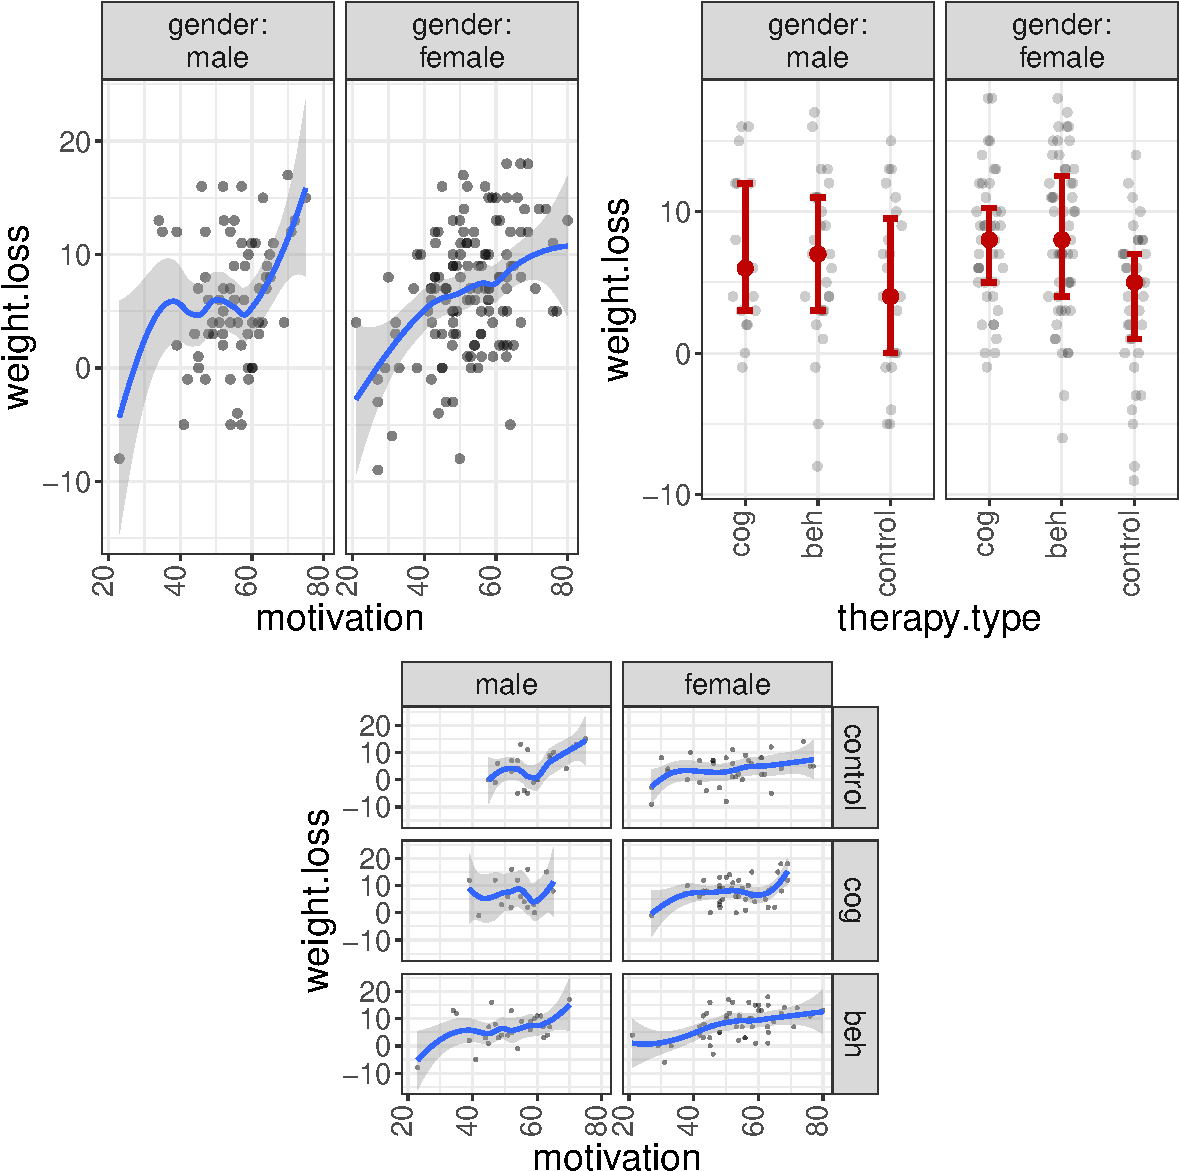
\includegraphics{flexplot_psychmeth_files/figure-latex/panels-1.pdf}
\caption{\label{fig:panels}A multivariate plot where \texttt{therapy.type} and \texttt{gender} are now shown in panels. \label{fig:panels}}
\end{figure}

\normalsize

\hypertarget{binning}{%
\subsection{Binning}\label{binning}}

Within \texttt{flexplot}, any numeric predictor, with the exception of the variable in the first slot, will be binned into discrete categories. These bins will then be represented in panels (if the variable is in the third or fourth slot) or as colors/symbols/lines (if the variable is in the second slot). The user has the option of specifying the number of bins (e.g., 2 or 3), or the user can specify breakpoints at which to bin. When the user specifies bins, \texttt{flexplot} will attempt to have an equal number of datapoints in each bin. However, \texttt{flexplot} may be unable to bin into the specified number of bins. For example, if a user specifies four bins, it is possible the scores at the 50th and 75th percentile are the same. In these cases, \texttt{flexplot} will choose a smaller bin number, though it will report such to the user. \texttt{flexplot} defaults to three bins.

When specifying breakpoints, the panels can have different sample sizes in each bin. A user may wish to do this if these breakpoints are meaningful (e.g., when particular scores are clinically meaningful, such as Beck Depression Inventory scores above 29 are considered severly depressed).

Whether using breakpoints or bins, the user can also specify labels for the bins. Figure \ref{fig:panels2} shows three plots of the same variables: the first specifies two breakpoints, the second specifies breakpoints with labels, and the third just specifies the number of bins.

\small

\begin{Shaded}
\begin{Highlighting}[]
\NormalTok{a }\OtherTok{=} \FunctionTok{flexplot}\NormalTok{(weight.loss }\SpecialCharTok{\textasciitilde{}}\NormalTok{ motivation }\SpecialCharTok{|}\NormalTok{ satisfaction, }
             \AttributeTok{data =}\NormalTok{ exercise\_data, }
             \AttributeTok{breaks =} \FunctionTok{list}\NormalTok{(}\AttributeTok{satisfaction=}\FunctionTok{c}\NormalTok{(}\DecValTok{3}\NormalTok{,}\DecValTok{7}\NormalTok{)))  }\SpecialCharTok{+}
  \CommentTok{\# change font size to eliminate overlap}
    \FunctionTok{theme}\NormalTok{(}\AttributeTok{axis.text.x =} 
            \FunctionTok{element\_text}\NormalTok{(}\AttributeTok{size =} \DecValTok{12}\NormalTok{, }\AttributeTok{angle =} \DecValTok{90}\NormalTok{, }\AttributeTok{hjust=}\FloatTok{0.95}\NormalTok{,}\AttributeTok{vjust=}\FloatTok{0.5}\NormalTok{))}
\NormalTok{b }\OtherTok{=} \FunctionTok{flexplot}\NormalTok{(weight.loss }\SpecialCharTok{\textasciitilde{}}\NormalTok{ motivation }\SpecialCharTok{+}\NormalTok{ satisfaction, }
             \AttributeTok{data =}\NormalTok{ exercise\_data, }
             \AttributeTok{breaks =} \FunctionTok{list}\NormalTok{(}\AttributeTok{satisfaction=}\FunctionTok{c}\NormalTok{(}\DecValTok{3}\NormalTok{,}\DecValTok{7}\NormalTok{)), }
             \AttributeTok{labels =} \FunctionTok{list}\NormalTok{(}\AttributeTok{satisfaction=}\FunctionTok{c}\NormalTok{(}\StringTok{"low"}\NormalTok{, }\StringTok{"medium"}\NormalTok{, }\StringTok{"high"}\NormalTok{)))}
\NormalTok{c }\OtherTok{=} \FunctionTok{flexplot}\NormalTok{(weight.loss }\SpecialCharTok{\textasciitilde{}}\NormalTok{ motivation }\SpecialCharTok{+}\NormalTok{ satisfaction, }
             \AttributeTok{data =}\NormalTok{ exercise\_data, }
             \AttributeTok{bins =} \DecValTok{2}\NormalTok{) }
\end{Highlighting}
\end{Shaded}

\normalsize

\small

\begin{figure}

{\centering 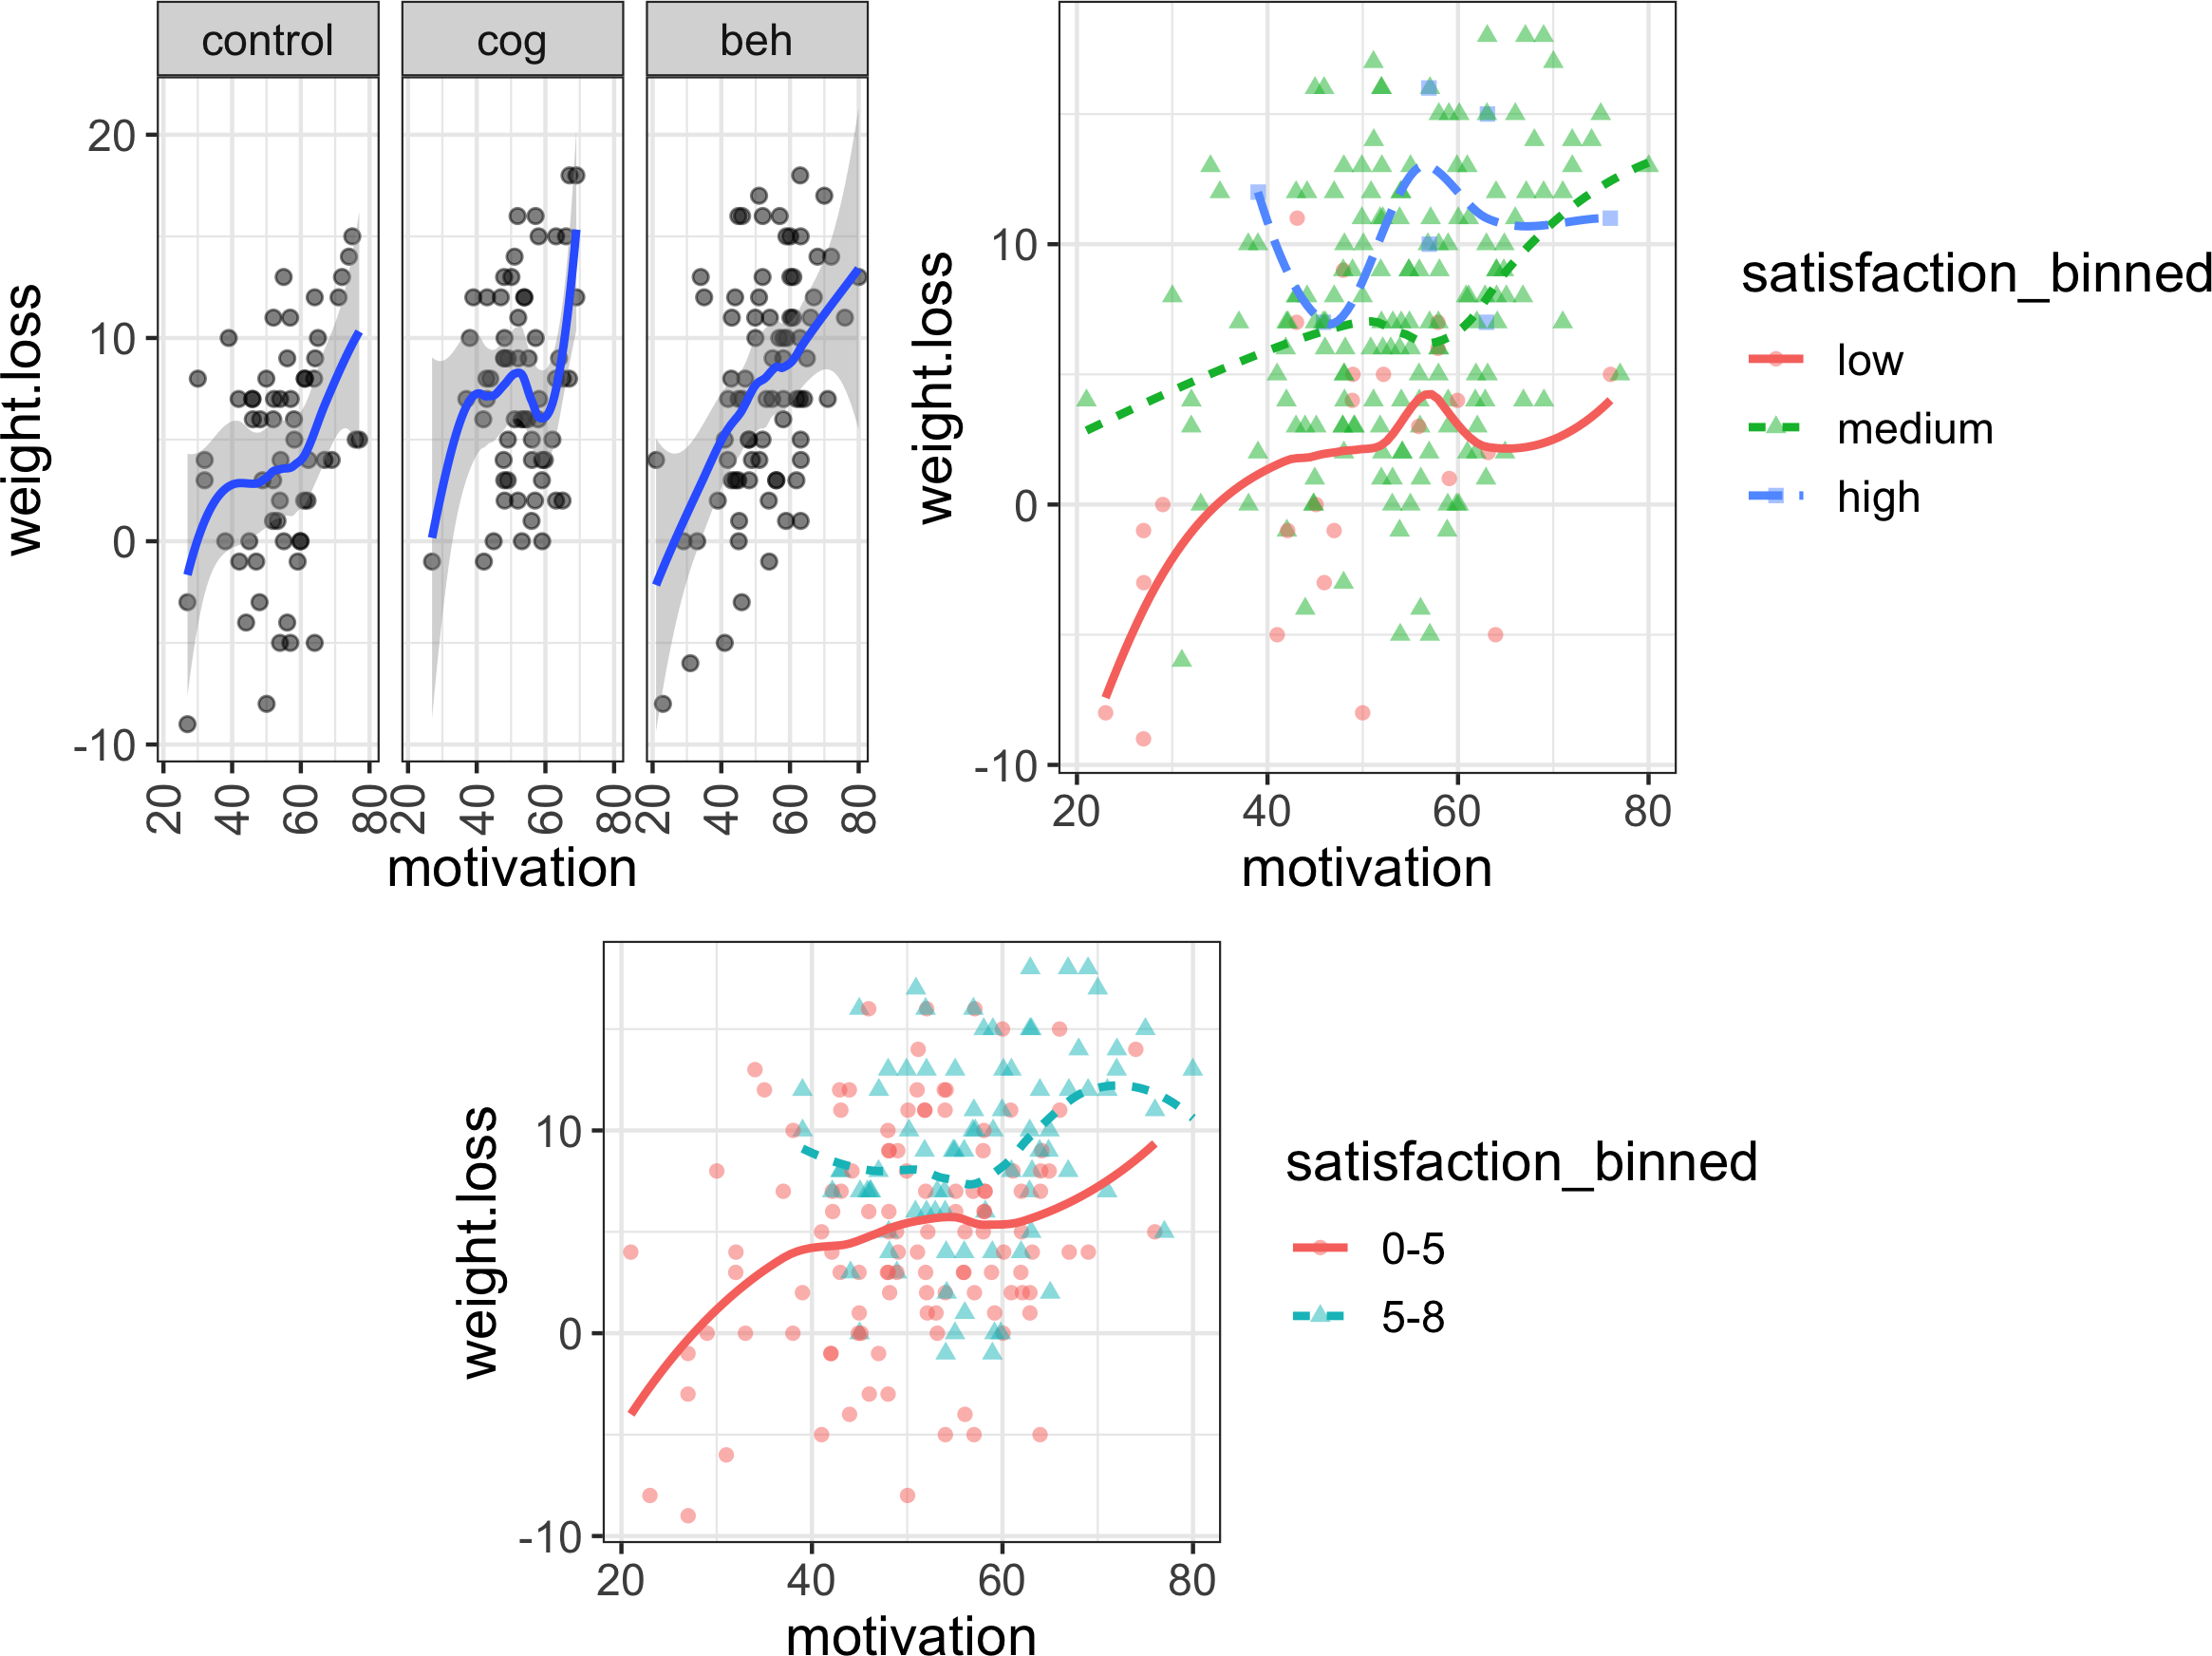
\includegraphics[width=1\linewidth]{flexplot_psychmeth_files/figure-latex/panels2-1} 

}

\caption{Plots reflecting choices of different break points (left-most plot), labels (right plot), and bins (bottom plot). \label{fig:panels2}}\label{fig:panels2}
\end{figure}

\normalsize

\hypertarget{ghost-lines}{%
\subsection{Ghost Lines}\label{ghost-lines}}

There are advantages and disadvantages to plotting a variable as a color/symbol/line versus panels. Panels reduce clutter, but make it harder to make comparisons because the eye has to travel further to make such comparisons. On the other hand, plotting in the same panel with different colors/lines/symbols means less visual distances to travel, but then there is too much clutter. One obvious solution is to stick with colors/symbols/lines and reduce transparency (or sample). However, there is a more innovative way of resolving this difficulty, by using something I call ghost lines. Ghost lines repeat the relationship from one panel to the other panels to make it easier to compare. Figure \ref{fig:ghost} demonstrates how to use ghost lines. By default, \texttt{flexplot} chooses the middle panel for odd numbers of panels, otherwise it chooses a panel close to the middle. The second line of code below specifies the referent panel by picking a value in the range of the referent panel. In Figure \ref{fig:ghost}, the ghost lines makes it clear that the relationship between \texttt{motivation} and \texttt{weight.loss} is stronger both at low and high levels of \texttt{satisfaction}, but less so at medium levels.

\small

\begin{Shaded}
\begin{Highlighting}[]
\CommentTok{\# change font size to eliminate overlap}
\FunctionTok{theme\_update}\NormalTok{(}\AttributeTok{axis.text.x =} 
            \FunctionTok{element\_text}\NormalTok{(}\AttributeTok{size =} \DecValTok{14}\NormalTok{))}
\FunctionTok{flexplot}\NormalTok{(weight.loss }\SpecialCharTok{\textasciitilde{}}\NormalTok{ motivation }\SpecialCharTok{|}\NormalTok{ satisfaction, }
             \AttributeTok{data =}\NormalTok{ exercise\_data, }\AttributeTok{method =} \StringTok{"lm"}\NormalTok{, }
             \AttributeTok{bins =} \DecValTok{3}\NormalTok{, }\AttributeTok{ghost.line =} \StringTok{"red"}\NormalTok{)}
\end{Highlighting}
\end{Shaded}

\begin{figure}

{\centering 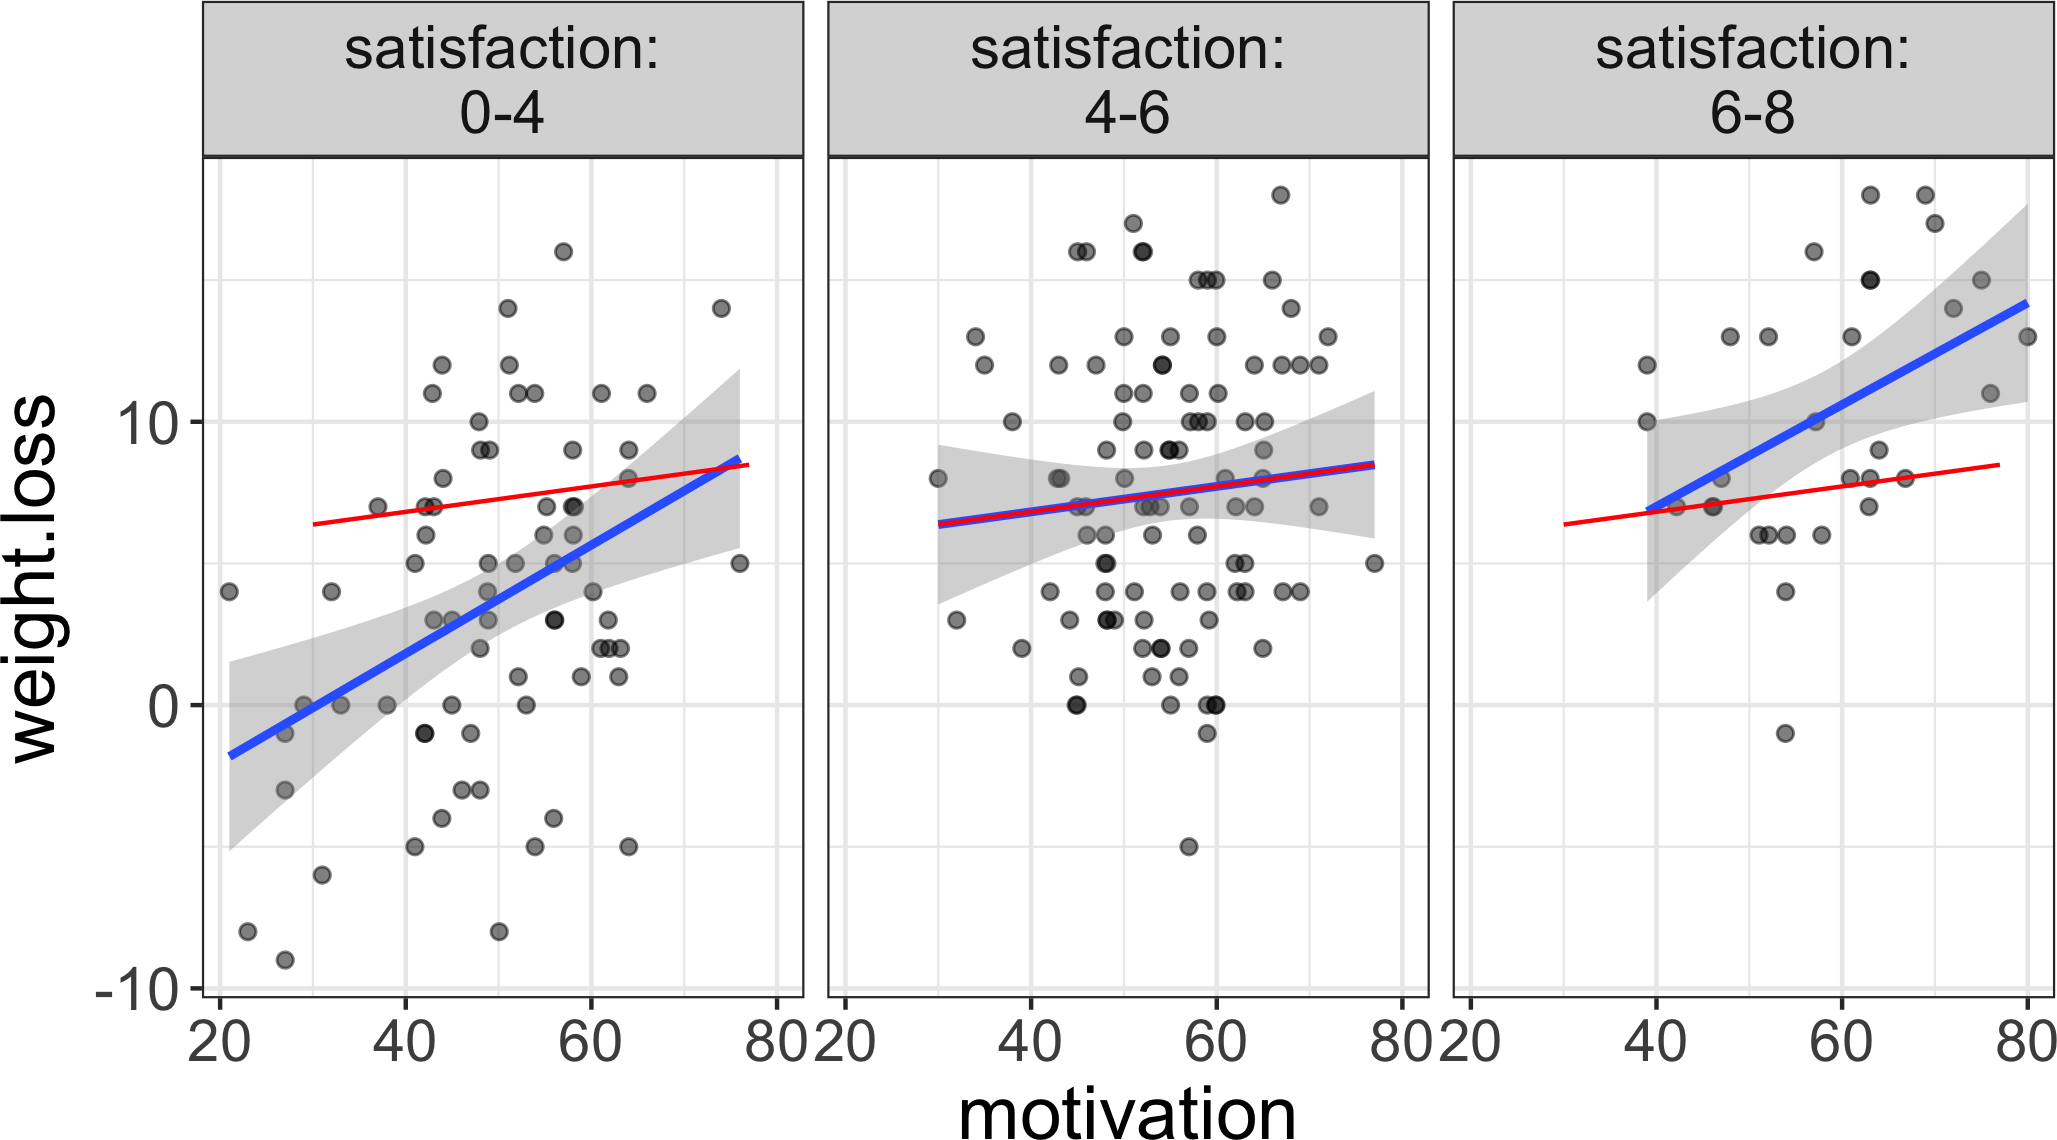
\includegraphics[width=0.8\linewidth]{flexplot_psychmeth_files/figure-latex/ghost-1} 

}

\caption{Ghost lines repeat the pattern from one panel to the others, making it easier to compare across panels. In this case, the line from the middle panel (Satisfaction = 4-6) is repeated in red across the other panels. \label{fig:ghost}}\label{fig:ghost}
\end{figure}

\normalsize

\hypertarget{general-strategy-for-plotting-multivariate-relationships}{%
\subsection{General Strategy for Plotting Multivariate Relationships}\label{general-strategy-for-plotting-multivariate-relationships}}

It is easy for multivariate graphs to become unnecessarily complicated. For example, the top image in Figure \ref{fig:threeway} shows a graphic where all four \texttt{flexplot} slots are occupied. This is very difficult to interpret. To simplify things, we could utilize several strategies. (See Fife, 2021 for a more detailed review of these and other strategies). First, we can specify two bins instead of the default three. We can also remove confidence intervals, reduce the opacity of the data, and plot regression lines.\footnote{These are great strategies to use \emph{after} one has determined that the model generally fits the data. If the data are curvilinear, for example, it would not make sense to plot straight lines or make the datapoints overly transparent.} Also, I generally try to have only two levels for the variable in the second slot (in this case, Male versus Female). Finally, we could add ghost lines. The bottom image in Figure \ref{fig:threeway} utilizes all these strategies and simplifies the visual interpretation immensely.

Another strategy is to mentally block out all panels but the diagonal (the bottom-left to top-right). The diagonal reflects the influence of \emph{both} variables as they increase (or decrease). In other words, they are a rough approximation of the average effect of the \(X1/Y\) relationship as you increase (or decrease) the paneled variables. If there is a general pattern of the lines consistently getting steeper (or shallower) as they move up the diagonal, that indicates there may be a three-way interaction effect. In Figure \ref{fig:threeway}, the lines seem pretty parallel going from bottom-left to top-right. The one thing that \emph{does} seem to change is that the colored lines go from below the ghost line to above it (indicating a main effect of \texttt{health} and/or \texttt{satisfaction}). In other words, we may be safe to do AVPs. However, before doing so, it may be best to combine graphs with statistical modeling.

\small

\begin{Shaded}
\begin{Highlighting}[]
\NormalTok{a }\OtherTok{=} \FunctionTok{flexplot}\NormalTok{(weight.loss }\SpecialCharTok{\textasciitilde{}}\NormalTok{ motivation }\SpecialCharTok{+}\NormalTok{ gender }\SpecialCharTok{|}\NormalTok{ satisfaction }\SpecialCharTok{+}\NormalTok{ health, }
    \AttributeTok{data =}\NormalTok{ exercise\_data) }
\NormalTok{b }\OtherTok{=} \FunctionTok{flexplot}\NormalTok{(weight.loss }\SpecialCharTok{\textasciitilde{}}\NormalTok{ motivation }\SpecialCharTok{+}\NormalTok{ gender }\SpecialCharTok{|}\NormalTok{ satisfaction }\SpecialCharTok{+}\NormalTok{ health, }
    \AttributeTok{data =}\NormalTok{ exercise\_data, }
    \AttributeTok{method =} \StringTok{"lm"}\NormalTok{, }\AttributeTok{se =}\NormalTok{ F, }\AttributeTok{bins =} \DecValTok{2}\NormalTok{, }\AttributeTok{ghost.line =} \StringTok{"black"}\NormalTok{, }\AttributeTok{alpha =}\NormalTok{ .}\DecValTok{2}\NormalTok{,}
    \AttributeTok{ghost.reference =} \FunctionTok{list}\NormalTok{(}\AttributeTok{satisfaction =} \DecValTok{0}\NormalTok{, }\AttributeTok{health =} \DecValTok{10}\NormalTok{, }\AttributeTok{gender =} \StringTok{"male"}\NormalTok{))}
\NormalTok{a }\SpecialCharTok{+}\NormalTok{ b }\SpecialCharTok{+} \FunctionTok{plot\_layout}\NormalTok{(}\AttributeTok{ncol =} \DecValTok{1}\NormalTok{)}
\end{Highlighting}
\end{Shaded}

\begin{figure}
\centering
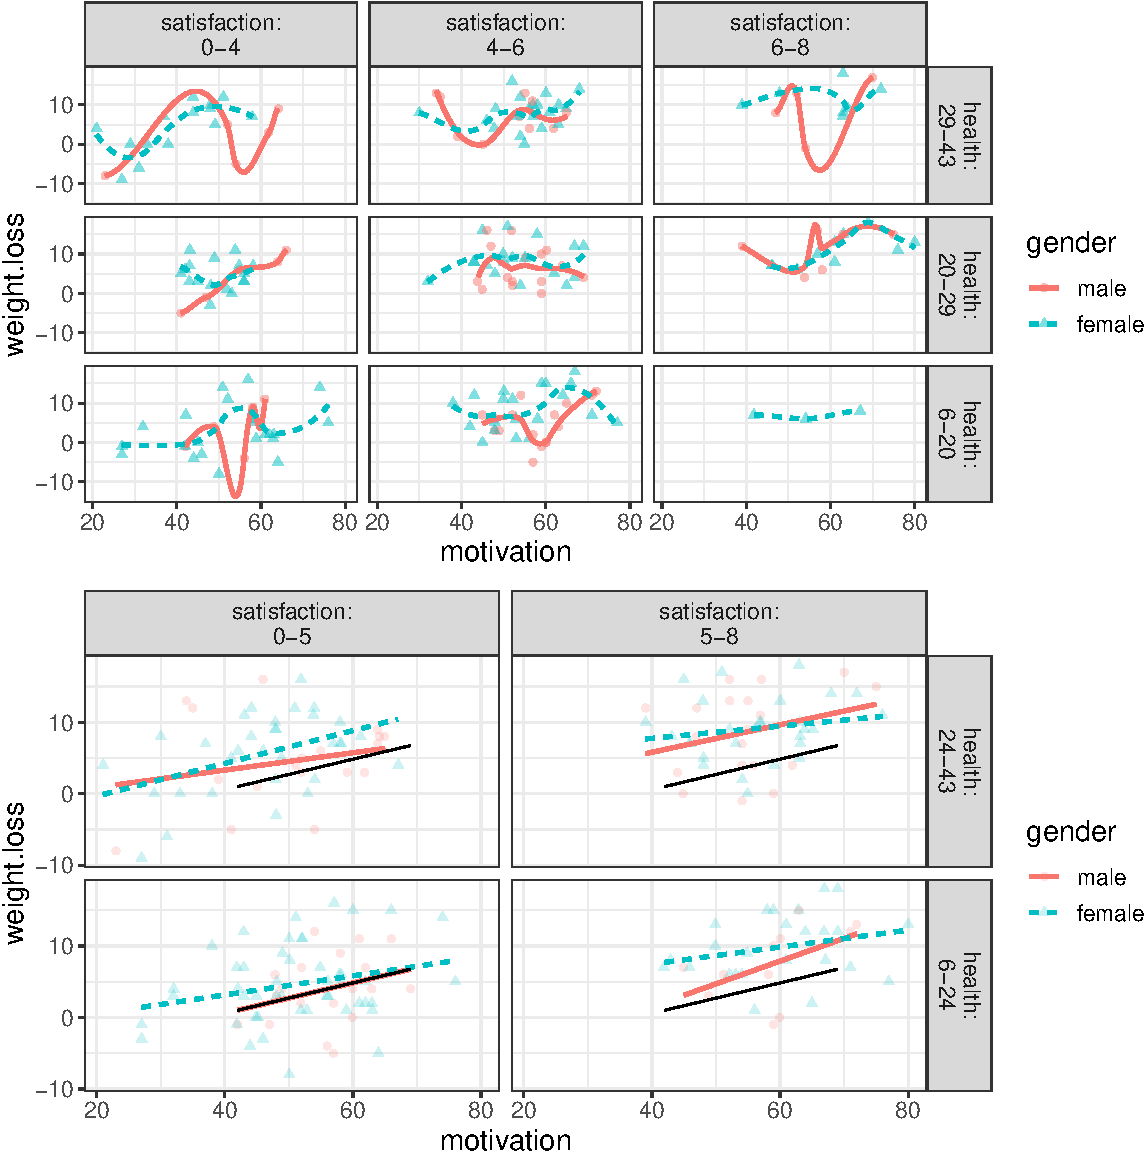
\includegraphics{flexplot_psychmeth_files/figure-latex/threeway-1.pdf}
\caption{\label{fig:threeway}Multivariate relationship between five variables. Each \texttt{flexplot} slot is occupied and it is difficult to interpret what is going on in the top figure, though the use of regression lines instead of loess lines, removing standard errors, reducing transparency of the datapoints, adding ghost lines, and reducing the number of bins have made it easier to interpret (bottom image). \label{fig:threeway}}
\end{figure}

\normalsize

\hypertarget{combining-modeling-and-visualizations}{%
\section{Combining Modeling and Visualizations}\label{combining-modeling-and-visualizations}}

Graphs are great for conveying general trends and patterns. However, it can be difficult to make decisions based on graphics, particularly when the pattern is not striking. For example, in Figure \ref{fig:threeway}, I don't feel entirely comfortable rejecting the idea that there are no interactions present in the model. Statistics, on the other hand, put visual patterns into concrete numbers that assist with statistical decision-making. Furthermore, it is easy to engage in confirmation bias when viewing a graphic. Statistics provide a much-needed reality check. As such, the two, statistics and graphs, ought to proceed hand in hand. Fortunately, \texttt{flexplot} was designed to complement statistical analysis (and vice versa). More specifically, \texttt{flexplot} has two additional visualization functions that simplify modeling, as well as two functions dedicated to statistical analysis.

\hypertarget{the-visualize-function}{%
\subsection{\texorpdfstring{The \texttt{visualize()} Function}{The visualize() Function}}\label{the-visualize-function}}

As I've mentioned repeatedly, one of the primary purposes of \texttt{flexplot} is to provide visualization for statistical models. The \texttt{visualize()} function is designed to do exactly that. Much like \texttt{summary()}, or \texttt{coef()}, \texttt{visualize()} is an R method within \texttt{flexplot} that can be applied to diverse sorts of models, including \texttt{lmer}, \texttt{lm}, and \texttt{glm}. \texttt{visualize()} attempts to generate a graphic that matches the formula used in a fitted model. Not only will \texttt{visualize()} plot a graphic to match the analysis, but it will also show diagnostic plots. For example, if we were to fit an ANCOVA model, we could graph it as follows:

\small

\begin{Shaded}
\begin{Highlighting}[]
\NormalTok{model }\OtherTok{=} \FunctionTok{lm}\NormalTok{(weight.loss }\SpecialCharTok{\textasciitilde{}}\NormalTok{ motivation }\SpecialCharTok{+}\NormalTok{ therapy.type, }
           \AttributeTok{data =}\NormalTok{ exercise\_data)}
\FunctionTok{visualize}\NormalTok{(model)}
\end{Highlighting}
\end{Shaded}

\begin{figure}
\centering
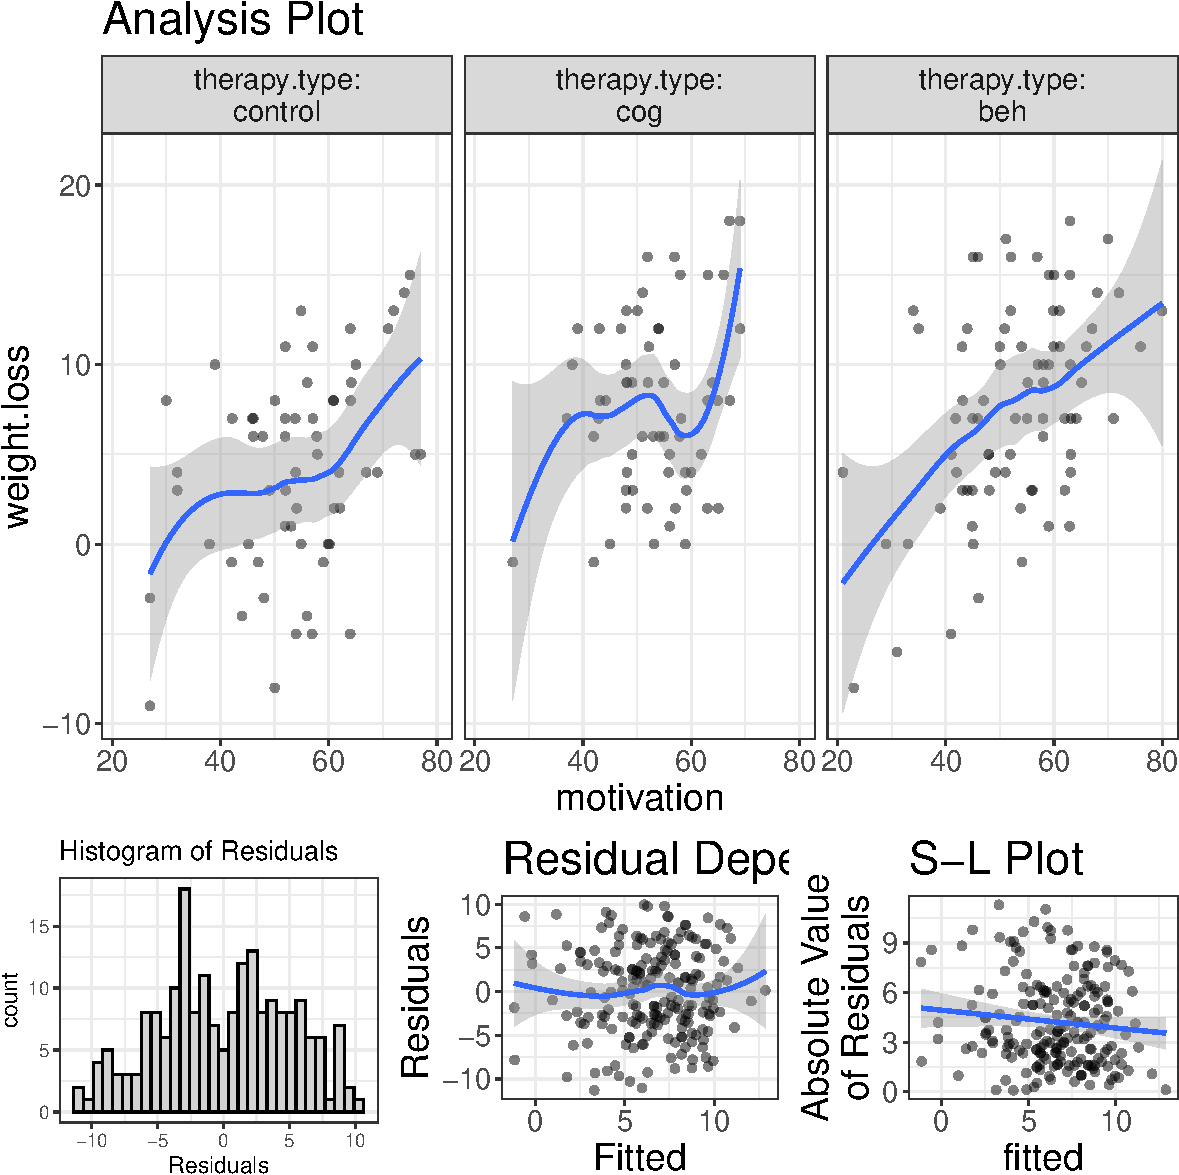
\includegraphics{flexplot_psychmeth_files/figure-latex/ancova-1.pdf}
\caption{\label{fig:ancova}Demonstration of the \texttt{visualize} function on a \texttt{lm} object. The top row shows a representation of the statistical model. The bottom row shows diagnostic plots. \label{fig:ancova}}
\end{figure}

\normalsize

For multivariate data, \texttt{visualize} will create a plot that will use panels and/or colors/symbols/lines. It will also generate diagnostic plots (histogram of the residuals, residual dependence plots, and S-L plots). The user can specify \emph{just} a plot of the model (\texttt{visualize(model1,\ "model")}), or \emph{just} a plot of the diagnostics (\texttt{visualize(model1,\ "residuals")}). Additionally, visualize can take \texttt{flexplot} arguments and even a \texttt{flexplot} formula.

\small

\begin{Shaded}
\begin{Highlighting}[]
\NormalTok{model }\OtherTok{=} \FunctionTok{lm}\NormalTok{(weight.loss }\SpecialCharTok{\textasciitilde{}}\NormalTok{ motivation }\SpecialCharTok{+}\NormalTok{ therapy.type, }\AttributeTok{data =}\NormalTok{ exercise\_data)}
\FunctionTok{visualize}\NormalTok{(model, }\AttributeTok{formula =}\NormalTok{ weight.loss }\SpecialCharTok{\textasciitilde{}}\NormalTok{ motivation }\SpecialCharTok{|}\NormalTok{ therapy.type, }
          \AttributeTok{ghost.line =} \StringTok{"gray"}\NormalTok{, }\AttributeTok{method =} \StringTok{"lm"}\NormalTok{, }\AttributeTok{plot =} \StringTok{"model"}\NormalTok{)}
\end{Highlighting}
\end{Shaded}

\begin{figure}
\centering
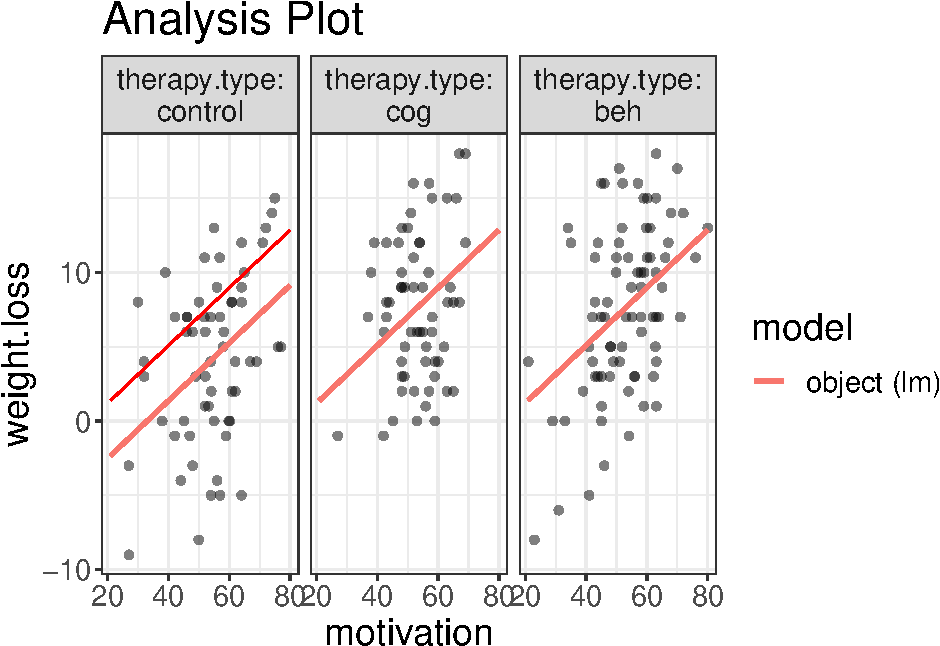
\includegraphics{flexplot_psychmeth_files/figure-latex/ancova2-1.pdf}
\caption{\label{fig:ancova2}Demonstration of the \texttt{visualize} function on a \texttt{lm} object, but with \texttt{flexplot} arguments controlling the output (as well as suppressing residuals). \label{fig:ancova2}}
\end{figure}

\normalsize

Figure \ref{fig:mixed} shows the \texttt{visualize()} function for a mixed model. With mixed models, \texttt{visualize()} randomly samples from the random effects (\texttt{Subject} in this case) and plots that as a variable in the graphic, and its location on the graph depends on whether the user specifies \texttt{formula}. If they do not, \texttt{visualize()} will default to placing it in the second slot (different lines/colors/shapes). This allows the user to graph a subset of the subjects in a mixed model to ensure the model chosen is appropriate.

\small

\begin{Shaded}
\begin{Highlighting}[]
\FunctionTok{require}\NormalTok{(lme4)}
\FunctionTok{data}\NormalTok{(math)}
\NormalTok{model }\OtherTok{=} \FunctionTok{lmer}\NormalTok{(MathAch }\SpecialCharTok{\textasciitilde{}}\NormalTok{ Sex }\SpecialCharTok{+}\NormalTok{ SES }\SpecialCharTok{+}\NormalTok{ (SES}\SpecialCharTok{|}\NormalTok{School), }\AttributeTok{data =}\NormalTok{ math)}
\FunctionTok{visualize}\NormalTok{(model, }
  \AttributeTok{plot =} \StringTok{"model"}\NormalTok{,}
  \AttributeTok{formula =}\NormalTok{ MathAch }\SpecialCharTok{\textasciitilde{}}\NormalTok{  SES }\SpecialCharTok{+}\NormalTok{ School}\SpecialCharTok{|}\NormalTok{ Sex, }
  \AttributeTok{sample =} \DecValTok{3}\NormalTok{)}
\end{Highlighting}
\end{Shaded}

\begin{figure}
\centering
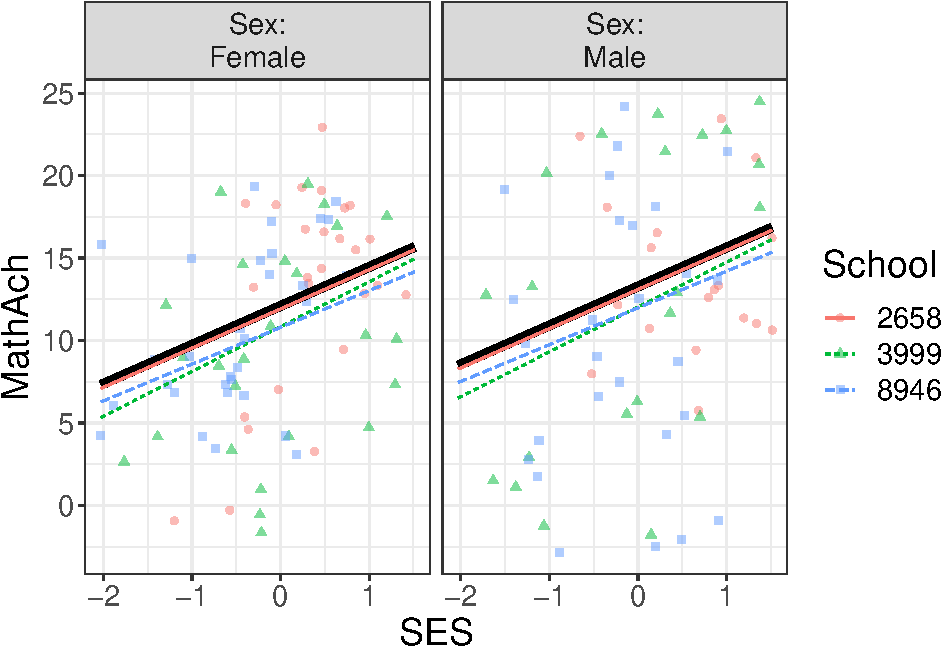
\includegraphics{flexplot_psychmeth_files/figure-latex/mixed-1.pdf}
\caption{\label{fig:mixed}Demonstration of the \texttt{visualize} function for a mixed model. In this graphic, each thin line represents the fit of a particular school. \label{fig:mixed}}
\end{figure}

\normalsize

\hypertarget{the-compare.fits-function}{%
\subsection{\texorpdfstring{The \texttt{compare.fits()} Function}{The compare.fits() Function}}\label{the-compare.fits-function}}

Very often in statistical modeling, we are interested in comparing two models (Rodgers, 2010), such as one with and one without an interaction term. There are many statistics available that allow easy comparison between models, such as the AIC, BIC, Bayes Factor, \(R^2\), p-values, etc. However, it is again important to \emph{see} how the two models differ in terms of fit. On multiple occasions, I have found various statistics show preference for one model, yet the graphs show the two models differ in only trivial ways.

That is where \texttt{compare.fits()} comes in. It is simply a wrapper for the \texttt{predict()} function, combined with the graphing capabilities of \texttt{flexplot}. More specifically, \texttt{compare.fits()} will overlay the fit of both models onto the raw data. For example, Figure \ref{fig:compare} shows the fit of two different models, one that includes an interaction and the other that does not. The arguments are very similar to \texttt{flexplot}, but with the addition of the model objects. Likewise, \texttt{compare.fits()} takes many of the same arguments. In this example, I've overlaid a black ghost line. Notice that the two lines (from \texttt{lm} and \texttt{interaction}) generate very similar predictions across the range of data, suggesting that a main effects model may be sufficient.

\small

\begin{Shaded}
\begin{Highlighting}[]
\NormalTok{model.me }\OtherTok{=} \FunctionTok{lm}\NormalTok{(weight.loss }\SpecialCharTok{\textasciitilde{}}\NormalTok{ motivation }\SpecialCharTok{+}\NormalTok{ therapy.type, }\AttributeTok{data =}\NormalTok{ exercise\_data)}
\NormalTok{model.int }\OtherTok{=} \FunctionTok{lm}\NormalTok{(weight.loss }\SpecialCharTok{\textasciitilde{}}\NormalTok{ motivation }\SpecialCharTok{*}\NormalTok{ therapy.type, }\AttributeTok{data =}\NormalTok{ exercise\_data)}
\FunctionTok{compare.fits}\NormalTok{(weight.loss }\SpecialCharTok{\textasciitilde{}}\NormalTok{ motivation }\SpecialCharTok{|}\NormalTok{ therapy.type, }
             \AttributeTok{data =}\NormalTok{ exercise\_data, model.me, model.int, }\AttributeTok{ghost.line =} \StringTok{"black"}\NormalTok{)}\SpecialCharTok{+}
  \CommentTok{\# get rid of variable name in panels (just put in the level)}
\NormalTok{      ggplot2}\SpecialCharTok{::}\FunctionTok{facet\_grid}\NormalTok{( }\SpecialCharTok{\textasciitilde{}}\NormalTok{ therapy.type, }
          \AttributeTok{labeller =}\NormalTok{ ggplot2}\SpecialCharTok{::}\FunctionTok{labeller}\NormalTok{(}\AttributeTok{therapy.type =}\NormalTok{ label\_value))}
\end{Highlighting}
\end{Shaded}

\begin{figure}
\centering
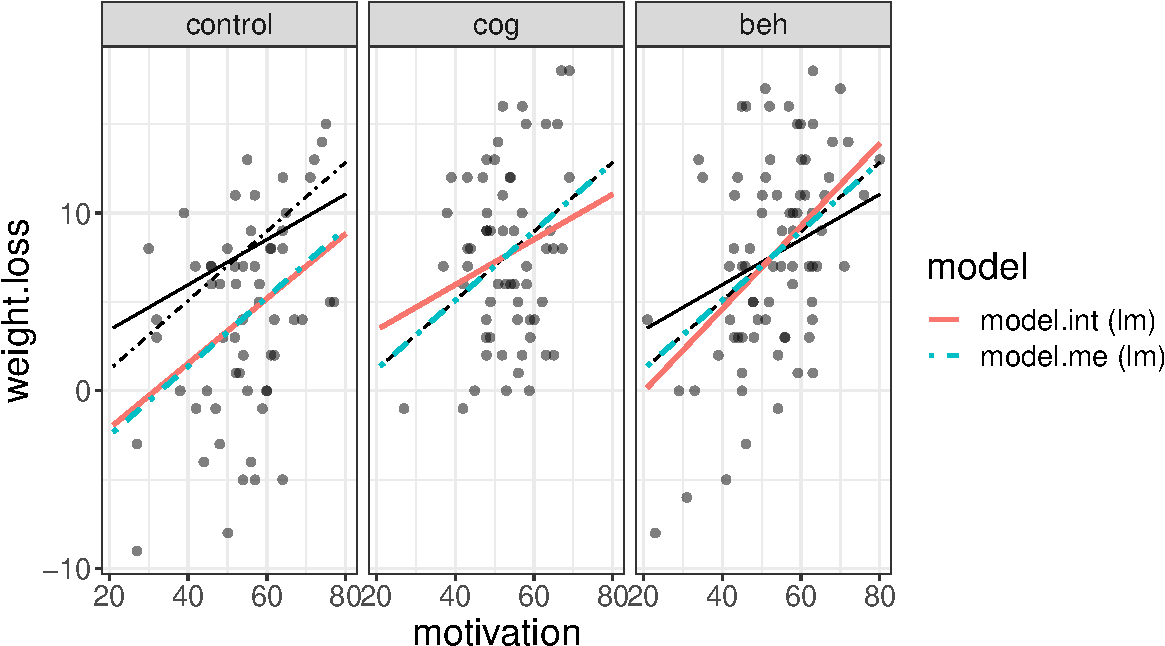
\includegraphics{flexplot_psychmeth_files/figure-latex/compare-1.pdf}
\caption{\label{fig:compare}Demonstration of the \texttt{compare.fits()} function, comparing a main effects and an interaction model. Ghost lines have been added from the \texttt{cog} condition for easier comparison across panels. \label{fig:compare}}
\end{figure}

\normalsize

\hypertarget{functions-devoted-to-estimation}{%
\section{Functions Devoted to Estimation}\label{functions-devoted-to-estimation}}

The \texttt{flexplot} package specializes in visualization, providing easy-to-use tools for graphical data analysis. However, it also has a small collection of non-visual functions that can be used hand-in hand with graphs. These functions include the \texttt{estimates()} method and \texttt{model.comparison()}.

\hypertarget{the-estimates-method}{%
\subsection{\texorpdfstring{The \texttt{estimates()} Method}{The estimates() Method}}\label{the-estimates-method}}

The \texttt{estimates()} method was designed to report paremeter estimates and effect sizes. Much like \texttt{flexplot}, many of the decisions are made in the background. And like \texttt{visualize()}, \texttt{estimates()} takes a fitted object as input. \texttt{estimates()} will then determine which estimates are most appropriate. For grouping variables, \texttt{estimates()} will report means, mean differences, and cohen's \(d\), as well as 95\% confidence intervals. For numeric variables, \texttt{estimates()} will report the intercept, slopes, and standardized slopes, also with corresponding confidence intervals. Additionally, it will report the model \(R^2\), as well as the semi-partial \(R^2\) associated with each effect in the model, except when there are interactions in the model. (With interactions present, it does not make sense to interpret main effects, which is why \texttt{estimates()} only reports the semi-partial for the interaction effect).

\small

\begin{Shaded}
\begin{Highlighting}[]
\FunctionTok{estimates}\NormalTok{(model.int)}
\end{Highlighting}
\end{Shaded}

\begin{verbatim}
## Model R squared:
## 0.222 (0.12, 0.32)
## 
## Semi-Partial R squared:
##              motivation            therapy.type motivation:therapy.type 
##                   0.125                   0.091                   0.006 
## 
## Estimates for Factors:
##      variables  levels estimate lower upper
## 1 therapy.type control     4.09  2.81  5.38
## 2                  beh     7.86  6.74  8.99
## 3                  cog     7.74  6.46  9.02
## 
## 
## Mean Differences:
##      variables  comparison difference lower upper cohens.d
## 1 therapy.type beh-control       3.77  0.71  6.84     0.75
## 2              cog-control       3.65  0.77  6.54     0.72
## 3                  cog-beh      -0.12 -2.99  2.75    -0.02
## 
## 
## Estimates for Numeric Variables = 
##     variables estimate  lower upper std.estimate std.lower std.upper
## 1 (Intercept)    -5.77 -11.84  0.31         0.00      0.00      0.00
## 2  motivation     0.18   0.07  0.29         0.35     -0.33      1.03
\end{verbatim}

\normalsize
The estimates shown support the conclusions gleaned from Figures \ref{fig:ancova}-\ref{fig:ancova2}, as well as Figure \ref{fig:compare}, namely that the addition of the interaction likely is not improving the fit enough to consider keeping.

\hypertarget{the-model.comparison-function}{%
\subsection{\texorpdfstring{The \texttt{model.comparison()} Function}{The model.comparison() Function}}\label{the-model.comparison-function}}

The final function I will mention is the \texttt{model.comparison()} function. This is similar to the \texttt{anova()} function in base \texttt{R}, but it includes additional estimates, including AIC, BIC, and the BIC-derived Bayes Factor. Additionally, \texttt{model.comparison()} works on both nested and non-nested functions. When used on non-nested functions, it will only compute AIC, BIC, and Bayes Factor. Also, the \texttt{model.comparison()} function will report the quantiles of the \emph{differences} in prediction. The \texttt{model.comparison()} below compares the main effects and the interaction model. The last reported numbers indicate that the maximum difference in prediction between the two models is only about 1.76 pounds, while the median difference is only about a quarter of a pound, suggesting the predictions are quite similar. Also, all statistics (AIC, BIC, Bayes Factor, p-value, and probably \(R^2\)) support the more simplified main effects model.

\small

\begin{Shaded}
\begin{Highlighting}[]
\FunctionTok{model.comparison}\NormalTok{(model.int, model.me)}
\end{Highlighting}
\end{Shaded}

\begin{verbatim}
## $statistics
##                aic      bic bayes.factor     p   rsq
## model.int 1223.041 1246.129        0.010 0.487 0.222
## model.me  1220.523 1237.015       95.294       0.217
## 
## $predicted_differences
##    0%   25%   50%   75%  100% 
## 0.003 0.087 0.252 0.395 1.757
\end{verbatim}

\normalsize

\hypertarget{discussion}{%
\section{Discussion}\label{discussion}}

There's little doubt that psychology is undergoing a methodological revolution. Scholars are pushing with increased fervor for preregistration, larger sample sizes, open science practices, etc. This is a very good thing, but inevitably insufficient. Data can often be deceptive, especially when tortured into submission by standard analyses. Alongside emerging post-replication crisis practices, I advocate for greater use of visualizations. Graphs are the best, and sometimes the only way to allow data to speak for itself.

Traditionally, producing graphs has been a cumbersome and extraneous procedure, quite divorced from the actual analyses. In this paper, I have introduced \texttt{flexplot}. \texttt{flexplot} aims to automate much of the graphical analysis that accompany data analysis. These graphs, which are based on scientifically-derived principles of visual perception, promise to promote sound data analysis and enhance data decision-making.

To use \texttt{flexplot}, users can download and install the R package through github, at www.github.com/dustinfife/flexplot. Alternatively, a point-and-click version of flexplot can be accessed via JASP (through the visual modeling module) or through Jamovi (through the flexplot module). For additional information on using flexplot, visit the following YouTube playlist: \url{https://bit.ly/2Qn4yoi}

\newpage

\hypertarget{references}{%
\section{References}\label{references}}

\begingroup
\setlength{\parindent}{-0.5in}
\setlength{\leftskip}{0.5in}

\hypertarget{refs}{}
\begin{CSLReferences}{1}{0}
\leavevmode\hypertarget{ref-Abbott2012}{}%
Abbott, G. R., Do, M., \& Byrne, L. K. (2012). {Diminished subjective wellbeing in schizotypy is more than just negative affect}. \emph{Personality and Individual Differences}, \emph{52}(8), 914--918. \url{https://doi.org/10.1016/j.paid.2012.01.018}

\leavevmode\hypertarget{ref-anscombe1973graphs}{}%
Anscombe, F. J. (1973). Graphs in statistical analysis. \emph{The American Statistician}, \emph{27}(1), 17--21.

\leavevmode\hypertarget{ref-Breheny}{}%
Breheny, P., \& Burchett, W. (2017). {Visualization of Regression Models Using visreg}. \emph{The R Journal}, 56--71. \url{https://doi.org/10.32614/rj-2017-046}

\leavevmode\hypertarget{ref-Camargo2015}{}%
Camargo, K., \& Grant, R. (2015). {Public health, science, and policy debate: being right is not enough.} \emph{American Journal of Public Health}, \emph{105}(2), 232--235. \url{https://doi.org/10.2105/AJPH.2014.302241}

\leavevmode\hypertarget{ref-Cleveland1994}{}%
Cleveland, W. S. (1994). {Coplots, nonparametric regression, and conditionally parametric fits}. \emph{Lecture Notes-Monograph Series}, 21--36.

\leavevmode\hypertarget{ref-cohen_earth_1994}{}%
Cohen, J. (1994). {The earth is round (p {\textless{}} .05).} \emph{American Psychologist}, \emph{49}(12), 997--1003. \url{https://doi.org/10.1037/0003-066X.49.12.997}

\leavevmode\hypertarget{ref-Correll2015}{}%
Correll, M. A. (2015). \emph{{Visual Statistics}} (Doctoral Dissertation). University of Wisconsin-Madison.

\leavevmode\hypertarget{ref-eklund2012beeswarm}{}%
Eklund, A. (2012). Beeswarm: The bee swarm plot, an alternative to stripchart. \emph{R Package Version 0.1}, \emph{5}.

\leavevmode\hypertarget{ref-Fife2019e}{}%
Fife, D. A. (2020). {The Eight Steps of Data Analysis: A Graphical Framework to Promote Sound Statistical Analysis}. \emph{Perspectives on Psychological Science}, \emph{15}. https://doi.org/\url{https://doi.org/10.1177/1745691620917333}

\leavevmode\hypertarget{ref-fifeprp}{}%
Fife, D. A. (2021). Visual partitioning for multivariate models: An approach for identifying and visualizing complex multivariate dataset. \emph{PsyArxiv}. \url{https://doi.org/10.31234/osf.io/avu2n}

\leavevmode\hypertarget{ref-fife2020bb}{}%
Fife, D. A., Longo, G., Correll, M., \& Tremoulet, P. (2020). A graph for every analysis: Mapping visuals onto common analyses. \emph{Behavioral Research Methods}.

\leavevmode\hypertarget{ref-Fife2019d}{}%
Fife, D. A., Tremoulet, P., \& Longo, G. (2019). \emph{{Developing and Empirically Validating Flexplot: A Tool for Mapping Statistical Analyses into Graphical Presentation}}. Chicago, IL: American Psychological Association.

\leavevmode\hypertarget{ref-Gigerenzer2004}{}%
Gigerenzer, G. (2004). {Mindless statistics}. \emph{The Journal of Socio-Economics}, \emph{33}(5), 587--606. \url{https://doi.org/10.1016/J.SOCEC.2004.09.033}

\leavevmode\hypertarget{ref-Hansen}{}%
Hansen, C. D., Chen, M., Johnson, C. R., Kaufman, A. E., \& Hagen, H. (2014). \emph{{Scientific Visualization: Uncertainty, Multifield, Biomedical, and Scalable Visualization}}. London: Springer. Retrieved from \url{http://www.springer.com/series/4562}

\leavevmode\hypertarget{ref-Healy2014a}{}%
Healy, K., \& Moody, J. (2014). {Data Visualization in Sociology}. \emph{Annual Review of Sociology}, \emph{40}(1), 105--128. \url{https://doi.org/10.1146/ANNUREV-SOC-071312-145551}

\leavevmode\hypertarget{ref-hoekstra_are_2012}{}%
Hoekstra, R., Kiers, H., \& Johnson, A. (2012). {Are Assumptions of Well-Known Statistical Techniques Checked, and Why Not?} \emph{Frontiers in Psychology}, \emph{3}(137). \url{https://doi.org/10.3389/fpsyg.2012.00137}

\leavevmode\hypertarget{ref-inbar2007minimalism}{}%
Inbar, O., Tractinsky, N., \& Meyer, J. (2007). Minimalism in information visualization: Attitudes towards maximizing the data-ink ratio. In \emph{ECCE} (Vol. 7, pp. 185--188).

\leavevmode\hypertarget{ref-Kosslyn2006e}{}%
Kosslyn, S. M. (2006). \emph{Graph design for eye and mind}. New York, NY: Oxford University Press.

\leavevmode\hypertarget{ref-Levine2018}{}%
Levine, S. S. (2018). {Show us your data: Connect the dots, improve science}. \emph{Management and Organization Review}, \emph{14}(2), 433--437. \url{https://doi.org/10.1017/mor.2018.19}

\leavevmode\hypertarget{ref-marieb1992human}{}%
Marieb, E. N. (1992). Human anatomy and physiology. Redwood city. \emph{CA: Benjamin/Cummings Publishing Company, Ine}, \emph{1}(992), 306--307.

\leavevmode\hypertarget{ref-Otten2015}{}%
Otten, J. J., Cheng, K., \& Drewnowski, A. (2015). {Infographics And Public Policy: Using Data Visualization To Convey Complex Information}. \emph{Health Affairs}, \emph{34}(11), 1901--1907. \url{https://doi.org/10.1377/hlthaff.2015.0642}

\leavevmode\hypertarget{ref-pandey2015deceptive}{}%
Pandey, A. V., Rall, K., Satterthwaite, M. L., Nov, O., \& Bertini, E. (2015). How deceptive are deceptive visualizations?: An empirical analysis of common distortion techniques. In \emph{Proceedings of the 33rd annual ACM conference on human factors in computing systems} (pp. 1469--1478). ACM.

\leavevmode\hypertarget{ref-Pastore2017}{}%
Pastore, M., Lionetti, F., \& Altoè, G. (2017). {When one shape does not fit all: A commentary essay on the use of graphs in psychological research}. Frontiers Media S.A. \url{https://doi.org/10.3389/fpsyg.2017.01666}

\leavevmode\hypertarget{ref-ripley2013package}{}%
Ripley, B., Venables, B., Bates, D. M., Hornik, K., Gebhardt, A., Firth, D., \& Ripley, M. B. (2013). Package {`mass.'} \emph{Cran R}, \emph{538}.

\leavevmode\hypertarget{ref-rodgers_epistemology_2010}{}%
Rodgers, J. L. (2010). {The epistemology of mathematical and statistical modeling: a quiet methodological revolution}. \emph{The American Psychologist}, \emph{65}(1), 1--12. \url{https://doi.org/10.1037/a0018326}

\leavevmode\hypertarget{ref-semetko2012sage}{}%
Semetko, H. A., \& Scammell, M. (2012). \emph{The SAGE handbook of political communication}. Sage Publications.

\leavevmode\hypertarget{ref-Tay2016a}{}%
Tay, L., Parrigon, S., Huang, Q., \& LeBreton, J. M. (2016). {Graphical Descriptives: A Way to Improve Data Transparency and Methodological Rigor in Psychology}. \emph{Perspectives on Psychological Science}, \emph{11}(5), 692--701. \url{https://doi.org/10.1177/1745691616663875}

\leavevmode\hypertarget{ref-Tufte2001}{}%
Tufte, E. R. (2001). \emph{The visual display of quantitative information}. Cheshire, CT: Graphics press.

\leavevmode\hypertarget{ref-Tukey1990}{}%
Tukey, J. W., \& Tukey, P. A. (1990). \emph{{Strips Displaying Empirical Distributions: I. Textured Dot Strips}}. Bellcore.

\leavevmode\hypertarget{ref-Tyron1998}{}%
Tyron, W. W. (1998). {The inscrutable null hypothesis.} \emph{American Psychologist}, \emph{53}(7), 796--796. \url{https://doi.org/10.1037/0003-066X.53.7.796.b}

\leavevmode\hypertarget{ref-umanath1994multiattribute}{}%
Umanath, N. S., \& Vessey, I. (1994). Multiattribute data presentation and human judgment: A cognitive fit perspective. \emph{Decision Sciences}, \emph{25}(5-6), 795--824.

\leavevmode\hypertarget{ref-vessey1991cognitive}{}%
Vessey, I. (1991). Cognitive fit: A theory-based analysis of the graphs versus tables literature. \emph{Decision Sciences}, \emph{22}(2), 219--240.

\leavevmode\hypertarget{ref-Wainer2010}{}%
Wainer, H. (2010). {Prelude}. In J. Berkson (Ed.), \emph{Semiology of graphics: Diagrams, networks, maps} (2nd ed., pp. ix--x). Redlands, CA: ESRI Press.

\leavevmode\hypertarget{ref-Weissgerber2015}{}%
Weissgerber, T. L., Milic, N. M., Winham, S. J., \& Garovic, V. D. (2015). {Beyond Bar and Line Graphs: Time for a New Data Presentation Paradigm}. \emph{PLoS Biology}, \emph{13}(4). \url{https://doi.org/10.1371/journal.pbio.1002128}

\leavevmode\hypertarget{ref-Wickham2010}{}%
Wickham, H. (2010). {A Layered Grammar of Graphics}. \emph{Journal of Computational and Graphical Statistics}, \emph{19}(1), 3--28. \url{https://doi.org/10.1198/jcgs.2009.07098}

\leavevmode\hypertarget{ref-Wilkinson1999}{}%
Wilkinson, L. (1999). {Dot plots}. \emph{The American Statistician}, \emph{53}(3), 276--281.

\leavevmode\hypertarget{ref-Wilkinson1999a}{}%
Wilkinson, L., \& Task Force on Statistical Inference. (1999). {Statistical Methods in Psychology Journals: Guidelines and Explanations}. \emph{American Psychologist}, \emph{54}(8), 594--601.

\end{CSLReferences}

\endgroup


\end{document}
